\section{Résumé en français}
%%%%%%%%%%%%%%%%%%%%%%%%%%%%%%%%%%%%%%%%%%%%%%%%%%%%%%%%%%%%%%%%%%%%%%%%%%%
%%%%%%%%%%%%%%%%%%%%%%%%%%%%%%%%%%%%%%%%%%%%%%%%%%%%%%%%%%%%%%%%%%%%%%%%%%%
Après avoir développé et analysé une simulation originale des grandes structures turbulentes dans le détroit de Gibraltar, dans le cinquième et dernier chapitre de ce manuscrit nous abordons la problématique de l'évaluation du mélange turbulent dans une simulation numérique des grandes structures turbulentes. La quantification et la localisation de ce mélange turbulent via celle des flux diapycnaux dans l'océan est un problème délicat. Les premières pierres d'un cadre théorique rigoureux ont en effet été posées il y a maintenant plus d'un demi-siècle par E. Lorenz \citep{lorenz_available_1955} avant qu'un algorithme simple ne soit proposé à la fin du siècle précédent par \cite{winters_available_1995} à partir d'une analyse appuyée sur une raisonnement très physique. La simplicité de cette application algorithmique en fait la force mais aussi d'une certaine façon la faiblesse, en particulier à cause des hypothèses très fortes sur lesquelles elle est fondée. Une hypothèse simplificatrice centrale est celle de la constance du volume de fluide considéré, hypothèse qui devient problématique lorsque le domaine considéré pour le bilan d'énergie potentielle est constitué de colonnes d'eau de mer dont la surface libre et donc la hauteur évoluent au cours du temps.

Une équation d'évolution complète a été proposée dans le cadre du chapitre \ref{chap2}, cette équation intègre en particulier la somme des contributions de la variation de surface en $dz^*/dt$ ($z^*(\rho)$ représentant ici la cote d'une particule de masse volumique $\rho$ dans le profil de référence réarrangé. A partir de cette équation d'évolution, l'algorithme classique proposé par \cite{winters_available_1995} est généralisé à une somme de colonnes océaniques: une diffusivité efficace est ainsi calculée à partir d'un bilan complet d'énergie potentielle (plus spécifiquement d'énergie potentielle de référence ou BPE en anglais) via la relation \ref{eq_kappaEff}.

Cet algorithme généralisé est ensuite appliqué à un ensemble de configurations de complexité croissante, chaque configuration permettant d'analyser et d'évaluer la pertinence de la quantification et de la localisation du mélange turbulent. Une équation d'advection-diffusion d'un traceur passif est tout d'abord étudiée dans le cadre de stratifications linéaires puis "bi-couche". Le mélange induit par les oscillations libres d'une cuve stratifiée ou le mélange induit dans un écoulement bi-couche instable ou par un écoulement dans la région du détroit de Gibraltar est lui-aussi analysé. Ces trois dernières configurations sont simulées numériquement avec le code océanique à toit libre CROCO dans sa version compressible et non-hydrostatique.

Une première conclusion est que la généralisation de l'algorithme de \cite{winters_available_1995} permet une évaluation rigoureuse et "suffisamment" précise du mélange turbulent (comparé aux erreurs induites par son évaluation). L'efficacité de l'algorithme doit toutefois encore être optimisée avant que ce dernier ne soit appliqué à très haute résolution à des régions océaniques d'extension conséquente.

%%%%%%%%%%%%%%%%%%%%%%%%%%%%%%%%%%%%%%%%%%%%%%%%%%%%%%%%%%%%%%%%%%%%%%%%%%%
\section{Introduction}
%%%%%%%%%%%%%%%%%%%%%%%%%%%%%%%%%%%%%%%%%%%%%%%%%%%%%%%%%%%%%%%%%%%%%%%%%%%
In the present chapter \ref{chapBPE}, a substantial step is made toward the quantification of mixing in realistic ocean configurations. In the general presentation of the \textit{ocean model} of chapter \ref{chap2}, a general evolution equation for the Background Potential Energy (BPE) was derived in equation (\noparref{eq_evolBPE}) of section \ref{section_PE_chap2}. This evolution equation can be applied to a region of the ocean made of free-surface water columns, with apparition of a source term of BPE linked to movement of this free-surface. The objective is now to apply \citet{winters_available_1995}'s algorithm for the determination of the reference profile $z^*(\rho)$ to this evolution equation, as a tool to evaluate the turbulent mixing in realistic ocean configurations.

%In addition to the evaluation of several new terms in the evolution equation, 
The generalisation of this algorithm to realistic numerical ocean configurations introduces additional difficulties to take into account : (i) bathymetry variations, (ii) variations of grid-cell volume in terrain-following s-coordinates, and (iii) diffusive and advective fluxes through open boundaries. In particular for this last point, diapycnal fluxes associated in fine to mixing are known to be several orders of magnitude smaller than advective fluxes associated for instance to ocean tides, and computation of the term of the balance equation must be carried out while preserving a high accuracy.

%Propositions are made to overcome such algorithmic difficulties and a step is made toward an original evaluation of mixing in realistic ocean configurations.

The generalized algorithm proposed here consequently takes root in the "milestone" publication by \citet{winters_available_1995}. Lately \citet{saenz_estimating_2015} and \citet{tailleux_local_2018} proposed more efficient algorithms for the determination of the reference profile (see \S \ref{section_PE_chap2} of the manuscript for a review). These modifications have not yet been implemented because (i) the cases studied so far do not require too large computations, and (ii) \citet{winters_available_1995}'s approach is to be used as a reference and, as a consequence, needs to be first implemented. The aim of this chapter is not only to evaluate the relevance and efficiency of the method but also to point where the approach needs to be further refined.

In the present chapter, we first propose an extension of \cite{winters_available_1995}'s algorithm to a free-surface, non-flat ocean in section \ref{BPE_algo}. It is applied first in section \ref{section_numlab} to a simple advection - diffusion equation using homogeneous grid cells. In a second step, CROCO ocean model is implemented in test-case configurations of section \ref{section_CROCO_BPE}. Those configurations are of increasing complexity in term of bathymetry and dynamics; the last, more realistic configuration being the vertical section of Gibraltar Experiment (SimRef) studied in chapter \ref{chapGBR2D}.

%With this original algorithm, we investigate, quantify and localize the turbulent mixing induced when a simple passive tracer is (numerically) advected by a constant current and diffused at a constant (known) rate. In the last section, the turbulent mixing induced in an oscillating tank, in an area of ocean submitted to Kelvin-Helmholtz instabilities and in the region of the strait of Gibraltar is studied.

%%%%%%%%%%%%%%%%%%%%%%%%%%%%%%%%%%%%%%%%%%%%%%%%%%%%%%%%%%%%%%%%%%%%%%%%%%%
\section{Generalized algorithm to evaluate effective diffusivity}
%%%%%%%%%%%%%%%%%%%%%%%%%%%%%%%%%%%%%%%%%%%%%%%%%%%%%%%%%%%%%%%%%%%%%%%%%%%
\label{BPE_algo}
%\cite{winters_available_1995}'s algorithm to quantify turbulent mixing includes several steps:
The framework applied reflexively to each configuration of this chapter is comprised of the following steps : 
\begin{enumerate}
\setlength\itemsep{0pt}
\item The volume of available ocean water located below a given depth $V(z)$ is evaluated at all depths. For non-moving bathymetry cases, this step is carried out only once. 
\item At a given time, the \textit{reference} density profile $\rho^*(z)$ is obtained following \citet{winters_available_1995} by "re-arranging" the stratification, filling from bottom to top the total available ocean volume as determined in the previous step with water parcels of increasing density. In "small"-extend configurations (such as the 2D vertical sections of this chapter), this "rearrangement" does not incur too large computations.%To avoid too large computations (and waiting for more efficient implementations), this "reorganisation" is restricted to "small"-extend configurations (such as 2D vertical sections).% In a non-flat ocean region and a fortiori when using a terrain-following s-coordinates, this re-arrangement has to be carried out with care since the surface of the ocean at a given depth depends itself on the depth.
\item The depth of a given density $z^*(\rho,t)=z^*(\mathbf{x},t)$ can in turn be obtained as the inverse function of the reference, re-arranged density profile $\rho^*(z)$. 
\item The Background Potential Energy $BPE(t)$, together with its evolution in time and the RHS terms of equation \ref{eq_evolBPE}, can then be computed based on $z^*(\rho,t)$ for the ocean region considered.
\item An "effective" diffusivity $\kappa_{eff}$ can finally be evaluated in a chosen area based on the generalized evolution equation of BPE \ref{eq_evolBPE}.
\end{enumerate}

Indeed, in equation \ref{eq_evolBPE}, the horizontal and vertical diffusivities (respectively $\kappa_h$ and $\kappa_v$) are the two unknowns of the problem. Here they are considered as homogeneous for the volume of ocean to which the algorithm is applied. Furthermore, in most cases studied hereafter, diffusivity has to be chosen isotropic, leading to $\kappa_h=\kappa_v=\kappa$. Indeed, the balance equation only provides one equation and, as a consequence, it can only lead to the determination of one unknown diffusivity.
In this case, the effective diffusivity $(\kappa_{eff})$ can be obtained by reformulating the evolution equation \ref{eq_evolBPE} as :
\begin{subequations}
  \begin{alignat}{2}
  \displaystyle 
 	&\frac{d PE_B}{d t} &&= \quad \underbrace{g\int_x \int_{-1}^0 \rho h \frac{d z^*}{d t}\bigg\rvert_{xs} \ dx ds}_{\phi_{\zeta}}\\
 & && \quad \underbrace{ -g\bigg[ \int_{-1}^0 \rho h z^* u \ ds\bigg]_{x} - g\bigg[ \int_x\rho z^* v_s \ dx\bigg]_0^1}_{F_A} \\
 & && \quad +\kappa_{eff}\underbrace{\bigg[+ g \ \bigg[ \int_{-1}^0 h z^*  \frac{\partial \rho}{\partial x}\bigg\rvert_{ts} \ ds \bigg]_{x}
 + g  \ \bigg[ \int_x z^* \frac{1}{h} \frac{\partial \rho}{\partial s}\bigg\rvert_{tx} \ dx \bigg]_0^1\bigg] }_{F_D}\\
 & && \quad +\kappa_{eff}\underbrace{\bigg[- g \int_x \int_{-1}^0 h  \frac{d z^*}{d \rho} \frac{\partial \rho}{\partial x}\bigg\rvert_{ts}^2 \ dx ds 
 - g  \int_x \int_{-1}^0 \frac{1}{h} \frac{d z^*}{d \rho} \frac{\partial \rho}{\partial s}\bigg\rvert_{tx}^2 \ dx ds\bigg]}_{\phi_D}
\end{alignat}
\label{bilanBPEal}
\end{subequations}
In essence, the balance is first computed with $\kappa_{eff}=1 kg/m^3$ and both diffusive terms $\phi_D$ and $F_D$ have high values. An instantaneous evaluation of diffusivity is then given by:
\begin{equation}
\kappa_{eff} = \frac{\frac{dPE_B}{dt}-(\phi_{\zeta}+F_A)}{F_D+\phi_D}
\label{eq_kappaEff}
\end{equation}

The treatment of this evolution equation needs to be achieved with a particular care. Indeed, the term $(\phi_\zeta)$ associated to $dz^*/dt$ can hardly be evaluated directly. It is computed as the sum of terms (1), (2) and (3) in relation \ref{eq_evolBPE0} in order to maintain the required accuracy without adding to the computational cost.% Indeed the expression in equation \ref{buoyancyzstar} with $\partial \zeta / \partial t$ and the Heaviside function is otherwise associated to large relative errors requiring large computing resources.
%The aim of this chapter is not only to evaluate the relevance and efficiency of the method but also to point where the approach needs to be further refined.
%First a simple advection - diffusion equation is studied numerically using homogeneous grid cells. In a second step, CROCO ocean model is implemented in test-case configurations of increasing complexity, the last, more realistic configuration being the vertical section of Gibraltar Experiment (SimRef) studied in chapter \ref{chapGBR2D}.

Additionally, in the first test-cases presented and discussed in section \ref{section_numlab}, configurations are cyclic in both horizontal and vertical directions, so the formulation of equation \ref{bilanBPEal} retains advective and diffusive fluxes through the top and bottom boundaries.

%At the opposite, in the first test-cases presented and discussed hereafter, configurations are cyclic in both horizontal and vertical directions. As a consequence, both advective and diffusive fluxes through the vertical boundaries are possible and those fluxes are obviously computed to verify the exact balance of the RHS and LHS of relation \ref{eq_evolBPE}.\\

%%%%%%%%%%%%%%%%%%%%%%%%%%%%%%%%%%%%%%%%%%%%%%%%%%%%%%%%%%%%%%%%%%%%%%%%%%%
\section{Explicit and implicit mixing in an advection-diffusion equation}
%%%%%%%%%%%%%%%%%%%%%%%%%%%%%%%%%%%%%%%%%%%%%%%%%%%%%%%%%%%%%%%%%%%%%%%%%%%
\label{section_numlab}
The evolution of the explicit (physical) and (numerically induced) implicit mixing is first tackled in the 2D vertical section of a flow governed by an advection - diffusion equation. As indicated previously, to avoid the heavy numerical treatment of tracer fluxes through lateral boundaries, the configuration is chosen cyclic in both directions.

The advection - diffusion governing equation of a passive tracer field $\psi$ is given by:
\begin{equation}
\frac{\partial \psi}{\partial t} = -u\frac{\partial \psi}{\partial x} - w\frac{\partial \psi}{\partial z} + \kappa_{exp}^h \frac{\partial^2 \Psi}{\partial x^2} + \kappa_{exp}^v \frac{\partial^2 \psi}{\partial z^2}
\label{eqAdvDiff}
\end{equation}
with $\kappa_{exp}^{h,v}$ the given explicit (known) diffusion coefficient (for most cases $\kappa_{exp}^{h}=\kappa_{exp}^{v}$).
Total volume is supposed to remain constant so that the RHS term $\phi_{\zeta}$ integrates to zero. No cases with vertical velocity are presented ($v_s\ =\ 0$) so the second term of $F_a$ in \ref{bilanBPEal} is also zero.
Depending on the test-case considered, the initial field of passive tracer is either equal to $\psi_1(x)=cos(2\pi x/L_x)$ or to $\psi_2(x,z)=Re(e^{i2\pi x/L_x}e^{i 2 \pi z/L_z})$.

\subsection{Local diffusion test configuration $(BPE_{exp})$}
\color{red} Intervertir section advection et diffusion??? Nous n'en avons pas reparlé ce mercredi matin Margaux... mais j'en resterais là!\color{black}

The first implementation is that of a diffusive but advection-free flow ($U\ =\ 0m/s$). The main numerical parameters are given in table \ref{tab_NUMLAB_exp}.

\begin{table}[h]
        %\begin{minipage}{.6\textwidth}
        \centering
        \begin{tabular}{|c|c|c|}
                \hline
                Configuration $BPE_{exp}$ & \textit{Parameters}\\
                \hline 
                Numerical Model & Advection-diffusion equation of passive tracers\\
                $L_x$ & 30 m\\
                $L_z$ & 30 m\\
                $\Delta x$ & 0.5 m\\
                $\Delta z$ & 0.5 m\\
                $\Delta t$ & 10 s\\
                Time stepping & RK3 \\
                Diffusivity & $Left: \kappa_{exp}^h=\kappa_{exp}^v=10^{-5}\ m^2/s$. $Right: \kappa_{exp}^h=\kappa_{exp}^v=10^{-3}\ m^2/s$. \\
                Advection & none\\
                Initial field & $\psi(x, z,\ 0)=\psi_2(x,z)$\\
                \hline
        \end{tabular}
        \captionof{table}{ $BPE_{exp}$ configuration: numerical parameters.}
        \label{tab_NUMLAB_exp}
        %\end{minipage}
\end{table}
\begin{figure}[h!]
\centering
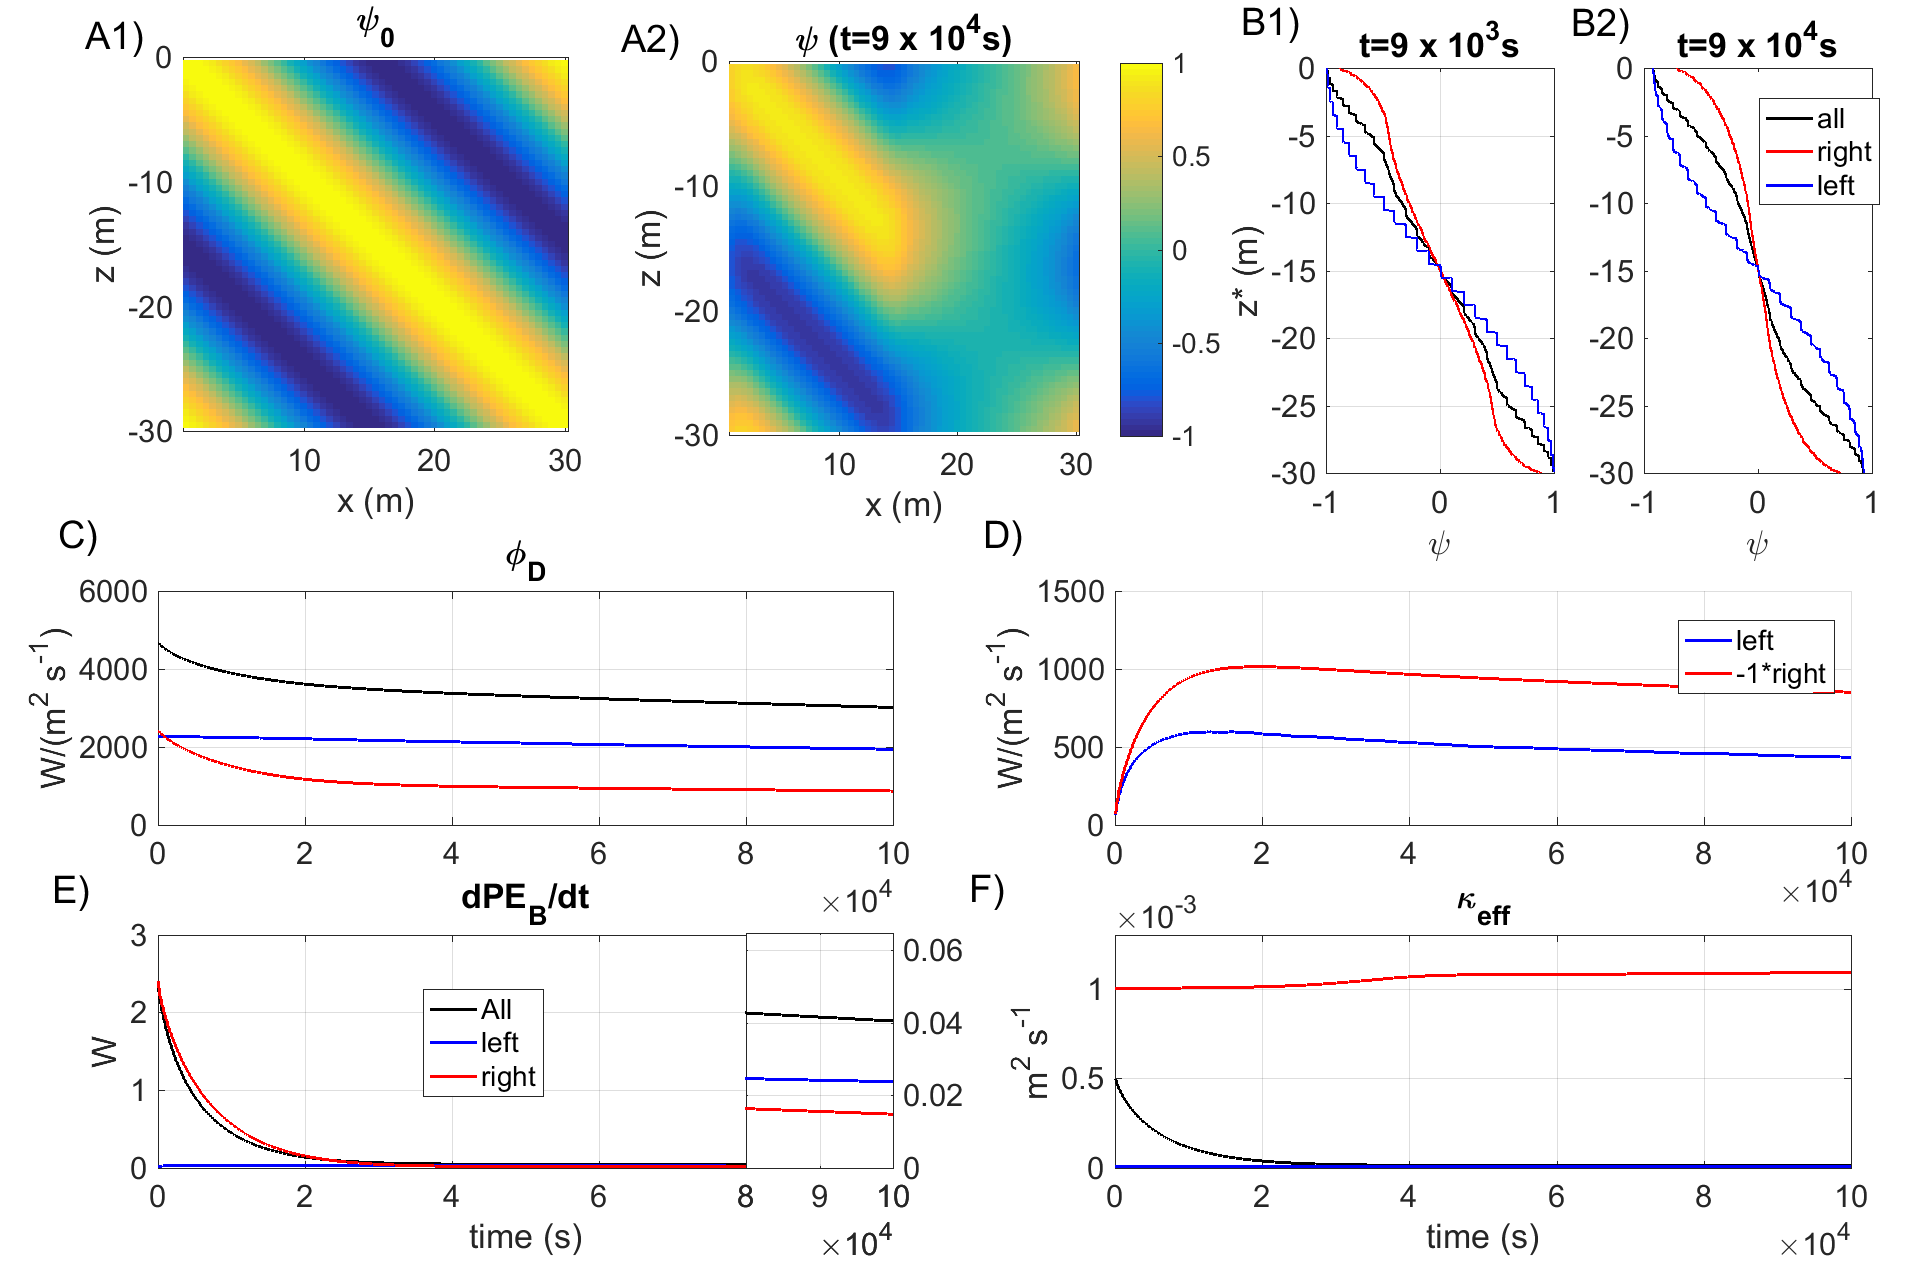
\includegraphics[width=1\textwidth]{./CHAP_BPE/AGBPE_numlab2_2.png}
\caption{(A1 and A2) Initial field of tracer $\psi$, and tracer field after $t=100s$ of simulation. (B1 and B2) Reference profiles $z^*(\psi)$ at $t=9.10^3s$ and $t=9.10^4s$ of simulation computed either with the fluid parcels of the left half sub-domain (blue), the right half sub-domain (red), or the complete domain (black). (C, D and E) RHS (C and D) and LHS (E) terms of equation \ref{bilanBPEal} computed on the different (sub-)domains. $F_D^{right}$ is indicated with a factor $-1$ in (D). (F) $\kappa_{eff}$ as evaluated in equation \ref{eq_kappaEff} with the previous terms on the different (sub-)domains.}
\label{fig2numlab}
\end{figure}
%Initial tracer field same as in fig \ref{fig1numlab}.
%\item Figure \ref{fig2numlab}. $dx=0.5$ m, $dz=0.5$ m, $L_x=30$ m, $L_z=20$ m, $dt=0.1s$. $\kappa_{exp}^x=\kappa_{exp}^z=\kappa_{exp}$ and $u=0$, no advection. RK3 timestepping scheme.
%\item For x$<$15 m, $\kappa_{exp} = 10^{-3}$, otherwise $\kappa_{exp} = 10^{-2}$ m$^2$/s.

The chosen initial passive tracer field is given by $\psi_2 (x,z)$ and is shown in figure (\noparref{fig2numlab}.A1).
To evaluate the capacity of the algorithm to deal with local variations of mixing (i.e. when the intensity of turbulent mixing is varying in space), the explicit diffusivity $\kappa_{exp}$ of equation \ref{eqAdvDiff} is non-homogeneous over the domain. It is one order of magnitude greater over the right half of the domain ($10^{-2}$ vs. $10^{-3} \ kg/m^3$ in the left half), so that as can be seen in figure (\noparref{fig2numlab}.A2) gradients are smoothed faster in this part of the grid.
The evaluation of $\kappa_{eff}$ presented in the previous section is carried out either for each half domain or for the whole domain. Three $z^*(\rho)$ reference profiles (respectively $z^*_{left}$, $z^*_{right}$ and $z^*_{all}$) are consequently computed with the "re-arrangement" algorithm considering only the fluid parcels in the left sub-domain, the right sub-domain, or the whole domain. Examples of those profiles are presented in figures (\noparref{fig2numlab}.B1 and B2).
Figures (\noparref{fig2numlab}.C to F) present the terms of equation \ref{bilanBPEal} computed from each reference profiles. It must be noted that neither the diffusive term $\phi_D$ nor the evolution of BPE $dPE_B/dt$ computed for the whole domain are equal to the sum of those terms computed on each half domain (for example $\phi_D^{all} \ne \phi_D^{left}+\phi_D^{right}$). This is due to the different definition of $z^*(\psi)$ depending of the domain extension chosen for the rearrangement. In the same way, the diffusive fluxes $F_D$ of figure (\noparref{fig2numlab}.D) do not cancel each other from one half domain to the other past the initialization as $z^*_{left}$ and $z^*_{right}$ diverge.
%In turn, the amplitude of the term $\phi_D$ varies depending if it is calculated for the latest $z^*_{all}$ reference profile or if it is obtained as the sum  $\phi_D^{left}+\phi_D^{right}$. The diapycnal fluxes $\phi_D^{left}$ and $\phi_D^{right}$ in this sum are themselves calculated respectively with the reference profiles $z^*_{left}$ or $z^*_{right}$. These fluxes do not cancel each other in so far as they are computed locally based on the local reference profiles of each sub-domain.
If the effective diffusivity $(\kappa_{eff})$ is evaluated over each half domain, figure (\noparref{fig2numlab}.E) shows that the algorithm provides the correct value of the diffusivity with: $\kappa_{eff}\approx\kappa_{exp}$. If $\kappa_{eff}$ is now evaluated over the whole domain, it is initially equivalent to the overall explicit mean diffusivity $(\kappa_{left}+\kappa_{right})/2$ but it decreases afterwards with time, approaching the value of $\kappa_{exp}^{left}$ after $t \approx 3.10^4s$. So the global effective diffusivity is finally close to the smallest value in the domain. The smallest value is associated with the half domain where gradients of the tracer field are at that time less affected by dissipation.
%, as diffusion is 'more efficient' on the right half of the domain,
%Because $\kappa_{eff}$ is computed as homogeneous, it must reflect the global diffusion process, however as time goes by in the simulation, diffusion is more efficient over the right half domain, for greater and greater $t$ the gradients of $\psi$ there will be smoothed out before   NON This can be explained by the differences in the re-arranged reference profiles. When this reference profile is computed "locally" (this is the case when the effective diffusivity is evaluated locally to compute $\kappa_{right}$, it is smoothed out quicker. As a consequence, the evaluated diapycnal flux decreases.\color{black}
%As time goes on, the effective diffusivity 
%\color{red} $\kappa_{eff}$ tends to the lowest value of diffusivity since in the right half (left or right ?),
%the vertical gradient of $\psi$ will be deteriorated quicker, hence the term of the integrand is smaller and the higher value of the gradient of $\psi$ in the left half will... (je n'arrive pas à formuler : l'évolution pilotée par là où le coef est le plus bas une fois que les gradients à droite sont résorbés)
%\item only able to differentiate for $\kappa(x)$.
%If diffusion coefficient was made to vary along the vertical direction, in the same way that when evaluate $\kappa_{eff}$ for the whole domain, integrates all contributions to the change in $z^*$ in the water column
%Explique plus simplement en français... cette étude est un peu loin maintenant... Au pire, on le rédige ensemble lundi matin.


\subsection{Implicit diffusion case $(BPE_{imp})$}
The same flow configuration is now investigated with homogeneous $\kappa_{exp}$ when advection is not neglected anymore ($u \ne 0$, table \ref{tab_NUMLAB_imp}).
\begin{table}[h]
        %\begin{minipage}{.6\textwidth}
        \centering
        \begin{tabular}{|c|c|c|}
                \hline
                Configuration $BPE_{imp}$ & \textit{Parameters}\\
                \hline 
                Numerical Model & Advection-diffusion equation of passive tracers\\
                $L_x$ & 30 m\\
                $L_z$ & 20 m\\
                $\Delta x$ & 0.5 m or 1.5 m\\
                $\Delta z$ & 0.5 m\\
                $\Delta t$ & 0.1 s\\
                Time stepping & RK3 \\
                Diffusivity & see text \\
                Advection & $U\ = 0.1\ m/s$ with UP1 or UP3 advective schemes.\\
                Initial field & With UP1 scheme: $\psi(x, z,\ 0)=\psi_2(x,z)$. \\
                 & With UP3 scheme: $\psi(x, z,\ 0)=\psi_1(x)$\\
                \hline
        \end{tabular}
        \captionof{table}{ $BPE_{imp}$ configuration: numerical parameters.}
        \label{tab_NUMLAB_imp}
        %\end{minipage}
\end{table}
%\item $dx=0.5$ m, $dz=0.5$ m, $L_x=30$ m, $L_z=20$ m, $dt=0.1s$ same as previously, but this time $U=0.1m/s$, and advection scheme either RK3-UP1 or RK3-UP3.
The objective with this new implementation is to evaluate the implicit diffusion $\kappa_{imp}$ due to upstream (UP1 or UP3) advective schemes. The effective diffusivity can be compared to the value obtained analytically for each upstream scheme. 

\subsubsection{First order upstream scheme (UP1)}
%Figure \ref{fig3numlab} shows the evolution of the implicit diffusivity obtained in the $BPE_{imp}$ configuration.
\begin{figure}[h!]
\centering
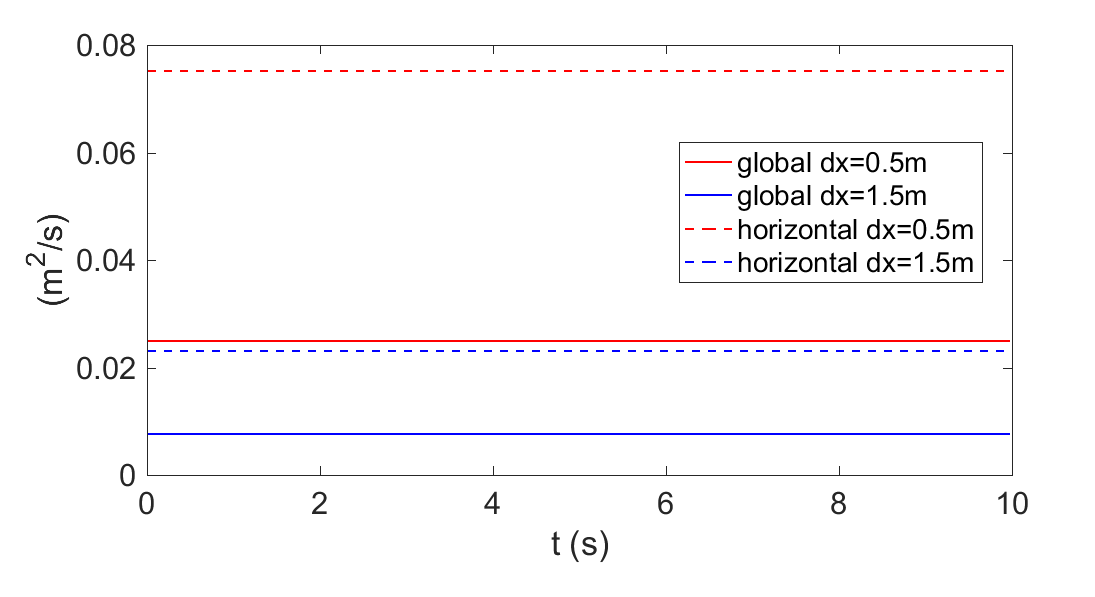
\includegraphics[width=0.5\textwidth]{./CHAP_BPE/AGBPE_numlab3.png}
\caption{$\kappa_{eff}$ computed in the case of implicit diffusion with RK3-UP1 scheme for $\Delta x=0.5m$ (red) or $\Delta x=0.1m$ (blue). In the computation of $\kappa_{eff}$, either isotropic diffusion is assumed ($\kappa_v=\kappa_h$, lines) or that diffusion is only applied in the horizontal direction ($\kappa_v=0$, dashed lines)}
\label{fig3numlab}
\end{figure}
The initial field is the same as in the previous $BPE_{exp}$ configuration ($\psi_2(x,z)$). Advective fluxes are now based on a first-order upstream scheme (UP1) and no explicit harmonic diffusion ($\kappa_{exp}=0$) is specified.
The modified equation for this discrete advection equation can be derived analytically:
\begin{equation}
\frac{\partial \psi}{\partial t}+U \frac{\partial \psi}{\partial x} = \frac{1}{2} U \Delta x  \frac{\partial^2 \psi}{\partial x^2} + \mathcal{O}(\frac{\partial^3 \psi}{\partial x^3})
\end{equation}
This leads to an analytical formulation of the implicit diffusion coefficient for the UP1 advective scheme: 
\begin{equation}
    \displaystyle
    \kappa_{h,imp}\approx\frac{1}{2}U \Delta x
\end{equation}
The implicit diffusivity consequently varies linearly with the grid scale and for $\Delta x\ =\ 0.5\ m$ (respectively $\Delta x\ =\ 1.5\ m$), it can reach $\kappa_{h,imp}\ =\ 0.025\ m^2/s$  (respectively $0.075\ m^2/s$).

Figure \ref{fig3numlab} shows that the correct value of the implicit diffusivity $(\kappa_{eff}=\kappa_{imp})$ can be recovered with the BPE algorithm only if the vertical component of the diffusion flux is not taken into account, i.e. when the along-flow diffusion flux only is considered. If both the horizontal and vertical components of the fluxes are retained in the evolution equation, the BPE algorithm leads to a smaller value of the effective diffusivity.
%Otherwise, the simulated evolution of the tracer field is assumed to come from isotropic diffusion in both vertical and horizontal direction, consequently $\kappa_{eff}$ is evaluated as lesser since there is this added contribution of vertical diffusion of equation \ref{bilanBPEal}. Note that it is possible to know that this latter hypothesis is wrong only because the model is specified to have no explicit diffusivity and only horizontal advection that induces numerical diffusion along this direction. 
\color{black}

%the value of $\kappa_{eff}$ is less than the analytically-computed implicit diffusivity. In this later case, the effective diffusivity is indeed supposed to be applied to both the horizontal and vertical components of the flow in equation \ref{bilanBPEal}.

\subsubsection{Third order upstream scheme (UP3)}
In this third configuration, the initial tracer field is now $\psi(x,\ 0)=\psi_1(x)$ (see figure \noparref{fig5numlab}.A).% in such a way that the solution of advection-diffusion problem can be computed analytically: $\psi(x,t)=e^{-\kappa k_x^2 t}cos(k(x-Ut))$ with $k_x=2\pi/L_x$.
A third-order upstream advective scheme (UP3) is now associated to the RK3 time-stepping with a non-vanishing horizontal velocity. The modified equation leads this time to a 4th-order diffusion term:
\begin{equation}
\frac{\partial \psi}{\partial t}+U \frac{\partial \psi}{\partial x} = \underbrace{\frac{1}{120}(5 C^3-10) U \Delta x^3}_{k_4}  \frac{\partial^4 \psi}{\partial x^4} + \mathcal{O}(\frac{\partial^5 \psi}{\partial x^5})
\end{equation}
where $C\ =\ U\Delta t/\Delta x$ is the advection Courant number. With $C=2 . 10^{-2}$ in the present configuration, the fourth order diffusivity takes the value $k_4\ =\ -1.10^{-3} m^4/s$. Note that the BPE algorithm conducted so far gives an implicit diffusion in form of a second-order diffusivity $k_2=\kappa_{eff}$.
This effective diffusivity is evaluated for several experiments relying on this configuration (table \ref{table_kappa}). In those experiments, in addition to the effect of the implicit diffusivity from the $UP3$ scheme, explicit harmonic diffusion is added, so that the effective diffusivity should be the sum of both contributions $\kappa_{eff} \approx \kappa_{exp} + \kappa_{imp}$.
The computed effective diffusivity show high-frequency oscillations with a non-negligible relative amplitude (not shown). Those oscillations are found regardless of the value of $\kappa_{exp}$. To filter out these oscillations, the value of $\kappa_{eff}$ indicated in table \ref{table_kappa} has been averaged over the whole simulation time. This is in agreement with the requirements of the treatment of the BPE evolution equation \ref{bilanBPEal} which requires that the effective diffusivity be computed over a period of time large enough with respect to the time-scale of the dissipation.
Once $\kappa_{exp}$ is removed from $\kappa_{eff}$, a unique value of $\kappa_{imp,2}$ is recovered at $4.65.10^{-5}\ m^2/s$ for all experiments.
%Several experiments are carried out with the configuration of schemes: in addition to the implicit diffusion induced by the upstream advection scheme, an explicit harmonic diffusion is also specified. 
%The effective coefficient found by BPE analysis consequently builds up to $\kappa_{eff} = \kappa_{exp} + \kappa_{imp}$.
%Figure \ref{fig5numlab}.b and table \ref{table_kappa} compare the effective diffusivity obtained with the BPE algorithm for several values of $\kappa_{exp}$. This diffusivity presents high-frequency oscillations with a non-negligible relative amplitude.
%\color{red}(correspond temps d'advection d'une cellule??? à vérifier (ou vient calcul des termes du bilan pas en RK3?))\color{black}. \\
%When averaged in time over the whole simulation, the effective diffusivity reaches approximately $4.65.10^{-5} m^2/s$ when $\kappa_{exp}\ =\ 0$. It is then evaluated for a series of configurations with non-zero explicit diffusivity and the (effective) implicit diffusivity $\kappa_{imp}$ is computed as the time-averaged effective diffusivity over the period minus the explicit diffusivity. The same  value of $4.65.10^{-5}\ m^2/s$ is recovered in all experiments.
%Since this value is for harmonic diffusion, the diffusion terms based on the effective second order diffusivity $(k_{imp,2}\ =\ \kappa_{eff}-\kappa_{exp})$ and on the analytical fourth-order diffusivity $k_4$ computed above can be compared in figure (\noparref{fig5numlab}.C) as factors of either the second or fourth order spatial derivate of $\psi$ taken at a random grid point. These terms are close to each other. 
To compare the effective second-order diffusivity $(k_{imp,2}\ =\ \kappa_{eff}-\kappa_{exp})$ with the analytical fourth-order diffusivity $k_4$, figure (\noparref{fig5numlab}.B) shows the evolution of the passive tracer field $(\psi)$ with the resulting second and fourth-order diffusion schemes. The resulting trends are close to each.
Note that the second-order and fourth-order advection terms do not operate in a similar way in wave-number space. Indeed, the fourth order is a more selective filter, smoothing more specifically small-scale gradients of passive tracer. This might be sufficient to explain the differences observed in figure (\noparref{fig5numlab}.B).
%\end{itemize}
\begin{table}[h!]
\centering
\begin{tabular}{|l|l|l|l|l|l|l|l|l|l|l|}
\hline
$\kappa_{exp}$ & $-10^{-4}$ &$-4.65.10^{-5}$ & $-10^{-5}$& $0$& $10^{-5}$& $10^{-4}$\\
\hline
$\kappa_{eff}$ & $-5.35.10^{-5}$ &$3.5.10^{-8}$ & $3.65.10^{-5}$& $4.65.10^{-5}$& $5.65.10^{-5}$& $14.65.10^{-5}$\\
\hline
$\kappa_{imp}$&\multicolumn{6}{c|}{$4.65.10^{-5}$}\\
\hline
\end{tabular}
\caption{Explicit coefficient given to simulation, effective coefficient computed from BPE analysis and implicit coefficient by deducting one from the other}
\label{table_kappa}
\end{table}

\begin{figure}[h!]
\centering
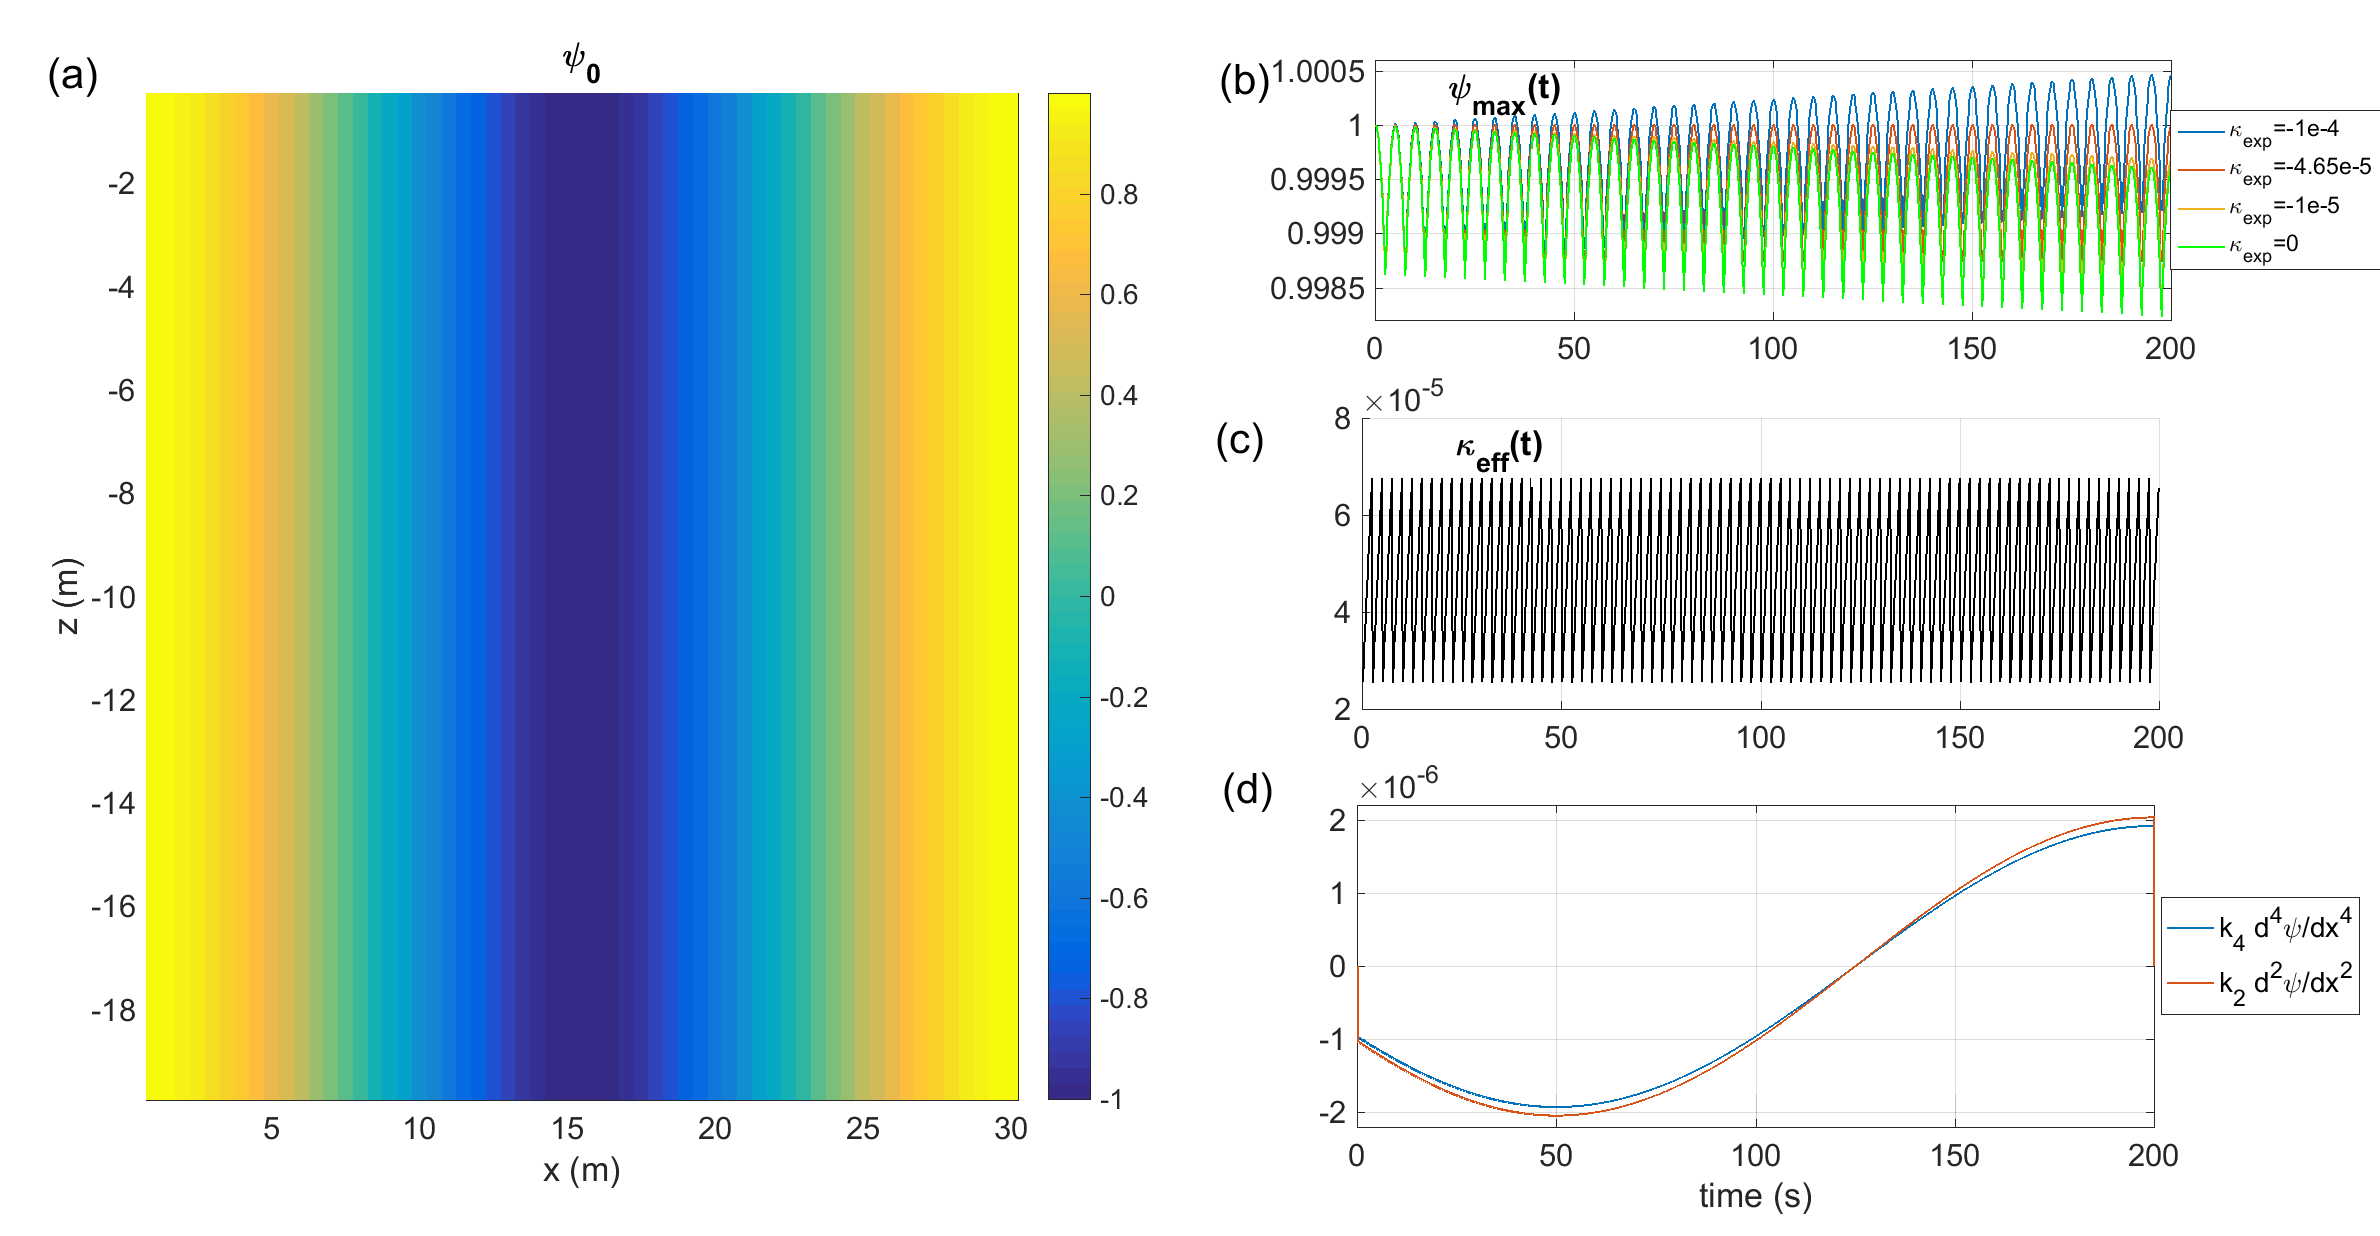
\includegraphics[width=1\textwidth]{./CHAP_BPE/AGBPE_numlab5.png}
\caption{(A) Initial tracer field. (B) Comparison of the fourth-order (with analytical value of the coefficient $k_4$) and second-order (with value of $k_2$ deduced from $\kappa_{eff}$ in table \ref{table_kappa}) formulation of diffusion at a random grid point.}
\label{fig5numlab}
\end{figure}

\subsection{Diffusion and advection timescales ($BPE_{ts}$)}
A third and last experiment ($BPE_{ts}$) based on the advection-diffusion equation of a passive tracer field is now presented to better understand the limitation of the BPE algorithm in terms of characteristic time and length scales. The idea is that the BPE algorithm can only give an accurate, valuable value of the effective diffusivity if (i) this diffusivity can be considered as homogeneous and can thus be extracted from the integral of the diapycnal flux in equation \ref{bilanBPEal} and (ii) diapycnal fluxes can be evaluated over time-scales (much) larger than the time-scale of the diapycnal fluxes at stake but also larger than the remaining dynamical time-scales in the studied ocean region.
Table \ref{tab_NUMLAB_ts} shows the physical and numerical parameters chosen for this experiment. The configuration is similar to $BPE_{exp}$ but both advection and diffusion are now active and the advection scheme is a second-order centered scheme (C2) known to lead to a vanishing implicit dissipation.\\
\begin{table}[h]
        %\begin{minipage}{.6\textwidth}
        \centering
        \begin{tabular}{|c|c|c|}
                \hline
                Configuration $BPE_{ts}$ & \textit{Parameters}\\
                \hline 
                Numerical Model & Advection-diffusion equation of passive tracers\\
                $L_x$ & 30 m\\
                $L_z$ & 30 m\\
                $\Delta x$ & 0.5 m\\
                $\Delta z$ & 0.5 m\\
                $\Delta t$ & 10 s\\
                Time stepping & RK3 \\
                Diffusivity & Left: $\kappa_{exp} = 10^{-5} \ m^2/s$. Right: $\kappa_{exp} = 10^{-3} \ m^2/s$.\\
                Advection & $U_1\ = 2.10^{-4}\ m/s$, $U_2\ =\ 2.10^{-3}\ m/s$ with C2 advective scheme.\\
                Initial field & $\psi(x,\ 0)=\psi_1(x)$\\
                \hline
        \end{tabular}
        \captionof{table}{$BPE_{ts}$ configuration: numerical parameters.}
        \label{tab_NUMLAB_ts}
        %\end{minipage}
\end{table}
\begin{figure}[h!]
\centering
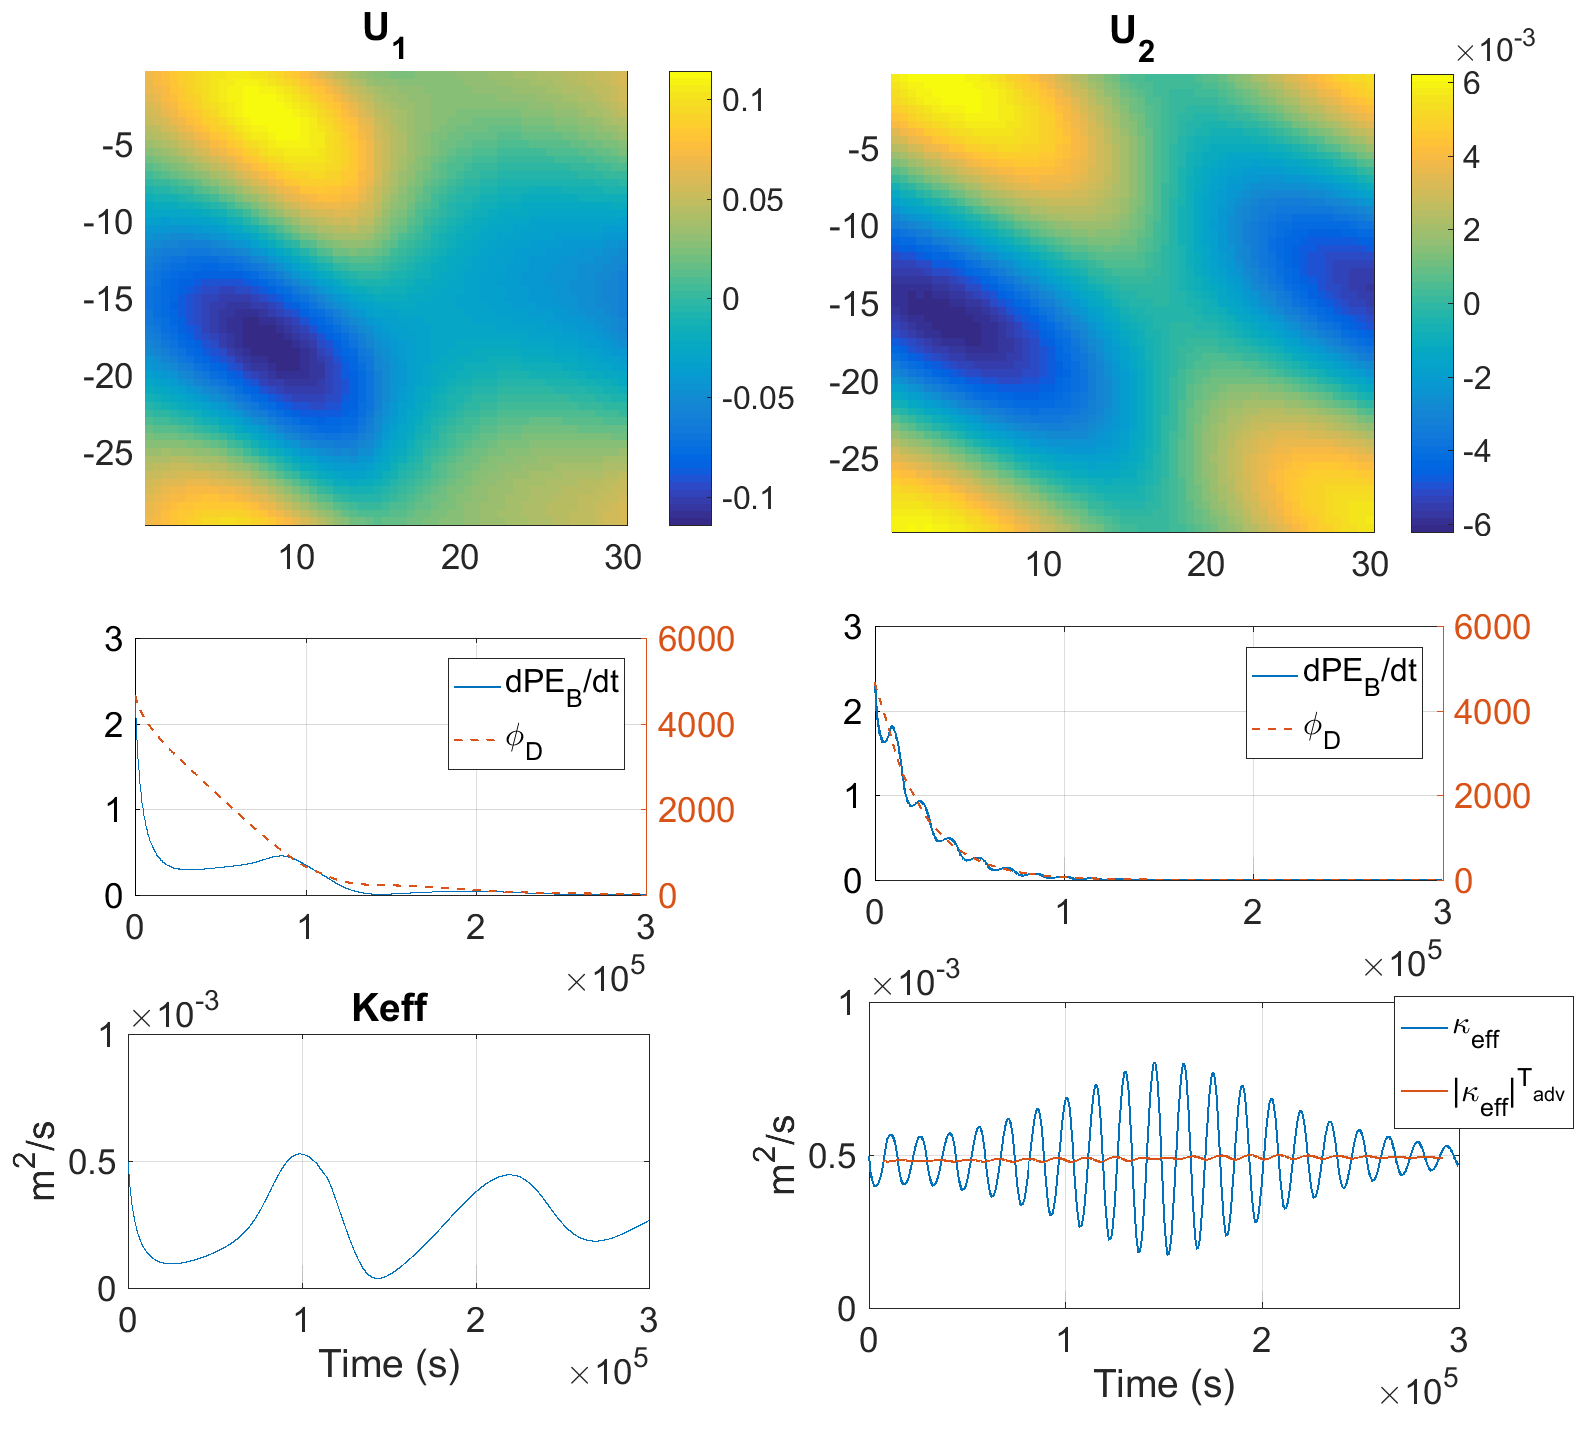
\includegraphics[width=1\textwidth]{./CHAP_BPE/Fig_numlab_advdiff3.png}
\caption{ }
\label{fig4numlab}
\end{figure}
%\begin{itemize}
%\item RK3-C2 scheme (no implicit diffusion). $\Delta x = \Delta z = 0.5m$, $L = H = 30m$, $dt=10s$
%\item $\kappa(x)$ avec $\kappa = 10^{-5} \ m^2/s$ for left half of domain and $\kappa = 10^{-3} \ m^2/s$ for right half. 
%\item Horizontal advection, two cases, either $U_1=2 \ 10^{-4} m/s $ or $U_2=2 \ 10^{-3} m/s $
Characteristic timescales are evaluated for advection, $(T_{adv}=L_{adv}/U)$, and for diffusion $(T_{\kappa}=L_{\kappa}^2/{\kappa})$, where L is the characteristic length-scale over which the flow is affected by each process. In this configuration, diffusion is supposed to be active over one half of the domain so $L_{\kappa}\ =\ 15\ m$ whereas advection occurs with the same exact value over the whole domain so that $L_{adv}\ =\ 30\ m$.\\
This leads to the following time-scales: $T_{\kappa}^{left}=2.25 \ 10^7 \ s$, $T_{\kappa}^{right}=2.25 \ 10^5 \ s$, and (depending on the value of $U$) $T_{adv}^{U_1}=1.5 \ 10^5 \ s$ or $T_{adv}^{U_2}=1.5 \ 10^4 \ s$. As a consequence:
\begin{equation}
\displaystyle
T_{adv}^{U_2}<<T_{adv}^{U_1}<T_{\kappa}^{right}<<T_{\kappa}^{left}
\end{equation}
Figure \ref{fig4numlab} shows the flow field after $t\ =\ 1.35\ 10^5 \ s$ for both values of the advective velocity. \\
For a small advective velocity $U\ =\ U_1$ (left), $t\ <\ T_{adv}^{U_1}$ and the displacement of the structure remains small compared to the initial field. When $t$ approaches $T_{\kappa}^{right}$ the smoothing by the explicit dissipation is much larger over the left half domain.\\ 
For a much larger advective velocity $U\ =\ U_2$ and after several advection time-scales $(t\ >>\ T_{adv}^{U_2})$, the tracer field remains symmetric
and the amplitude of the tracer-field variations are this time damped over the whole domain. This damping is higher than the damping induced by the smaller advective velocity field $(U_1)$ over the left part.
Figures (\noparref{fig4numlab}.e-f) additionally show the variations with time of the effective diffusivity $\kappa_{eff}$ for each advective velocity field over the whole domain. \\
%The average of the two values of explicit diffusivity prescribed over the whole domain is equal to $5 \ 10^{-4} \ m^2/s$.
With a small advective velocity fields $U_1$, the time-scales $T_{\kappa}^{right}$ and $T_{adv}^{U_1}$ are close to each other and the effective diffusivity is initially close to the prescribed averaged explicit diffusivity $(5 \ 10^{-4} \ m^2/s)$. At $t\ =\ 2.785\ 10^5 s$, i.e. after approximately two advective time-scales $T_{adv}^{U_1}$, all the fluid parcels have been advected through the high dissipation area.
As time goes on, this effective velocity shows oscillations over a period close to the advective time-scale. The effective diffusivity oscillates around a mean value twice as small as the average value of the prescribed explicit velocity. \\
%but after $t=3.86 \ 10^4 s$ , reach a minimum of $\kappa_{eff}=3.24 \ 10^{-5} m^2/s$. This value then increases again slowly then stabilizes at $\kappa_{eff}=2.2 \ 10^{-4} \ m^2/s$ after $t=2.785 \ 10^5 s$ approx half $T_{adv}^{U_1}$ at this point all original fluid parcels have been advected through the high dissipation area.
With a much larger advective velocity fields $U_2$ now, the effective diffusivity oscillates around the averaged explicit advective velocity. The time-scale of the oscillations is now smaller: it remains closer to the advective time-scale $T_{adv}^{U_2}$.
When the effective velocity is computed over each sub-domain, the expected values are recovered and this diffusivity oscillates over the same advective time-scale but with a much smaller amplitude. 

\subsection{Partial conclusion}
The various experiments carried out in the frame of this simple but rather complete advection-diffusion configuration confirms that \cite{winters_available_1995}'s BPE algorithm can lead to a quantification but also to a localization of the turbulent mixing coefficient in regional ocean configurations. Large variations of the effective diffusivity can yet be observed when it is evaluated over a period smaller than or close to time-scales of active process (such as the advective time-scale in the proposed experiments). To be accurate, this effective diffusivity must in any event be carried out over time-scale larger than the estimated time-scale of the diapycnal fluxes in the region of interest. The effective diffusivity thus calculated is to be viewed as an average for the region (viewed as a sum of water-columns) over which the evolution equation \ref{bilanBPEal} has been evaluated. It has also been confirmed that this algorithm can conveniently be used to evaluate the implicit dissipation induced by advective schemes.

%%%%%%%%%%%%%%%%%%%%%%%%%%%%%%%%%%%%%%%%%%%%%%%%%%%%%%%%%%%%%%%%%
\section{Toward an evaluation of mixing in real ocean}
%%%%%%%%%%%%%%%%%%%%%%%%%%%%%%%%%%%%%%%%%%%%%%%%%%%%%%%%%%%%%%%%%
\label{section_CROCO_BPE}
Several additional test configurations of increasing complexity are now presented to progress toward an evaluation of mixing in a "real ocean" with the "generalized" BPE algorithm presented in \S \ref{BPE_algo}. The consequences of the variations of the ocean free-surface are thus first explored in the case of the free oscillations of a stratified tank. Mixing is then finally evaluated with the BPE algorithm when Kelvin-Helmholtz instabilities are developing and in the region of Gibraltar strait.

\subsection{Free oscillations of a stratified tank ($BPE_{tank}$)}
As shown in \S \ref{section_PE_chap2}, the variations of the ocean free-surface induce several adaptations of the evolution equation of BPE and, as a consequence, they have a significant impact on the evaluation of mixing in realistic configurations. The present configuration focuses on the mixing induced by the natural (free) oscillations of a stratified tank initially subjected to a gradient of free-surface anomaly. The physical and numerical parameters are presented in table \ref{tab_BPE_TANK}.
\begin{table}[h]
        %\begin{minipage}{.6\textwidth}
        \centering
        \begin{tabular}{|c|c|c|}
                \hline
                Configuration $BPE_{tank}$ & \textit{Parameters}\\
                \hline 
                Numerical Model & CROCO (compressible, non-hydrostatic kernel)\\
                $L_x$ & 50 m\\
                $L_z$ & 10 m\\
                $\Delta x$ & 0.2 m\\
                $\Delta z$ & $\approx\ 0.2\ m$\\
                $\Delta t$ & close to CFL requirements in test-configurations\\
                Diffusivity & $\kappa_{exp} = 10^{-4} \ m^2/s$\\
                \hline
        \end{tabular}
        \captionof{table}{$BPE_{ts}$ configuration: numerical parameters.}
        \label{tab_BPE_TANK}
        %\end{minipage}
\end{table}
The initial perturbation of the ocean free-surface is chosen equal to:
\begin{equation}
\displaystyle
\zeta(x,t=0)=\zeta_0\ cos\left(\frac{\pi x}{L_x}\right)
\end{equation}
with $\zeta_0\ =\ 2\ mm$.
%Now apply determination of $\kappa_{eff}$ to numerical cases Based on TANK experiment (ref?), adapted to have stratification. Evolution of the density tracer field, through the complete system of equation for ocean CROCO. Closed domain, 2D. No initial velocity.
\subsubsection{Linear stratification and free surface: induced mixing}
The initial anomaly of the free-surface induces natural oscillations of the stratified flow in the tank due to the propagation and resonance of surface gravity waves. The induced currents lead to diapycnal fluxes and, as a consequence, they participate to increase turbulent mixing.\\ 
\begin{figure}[h!]
\centering
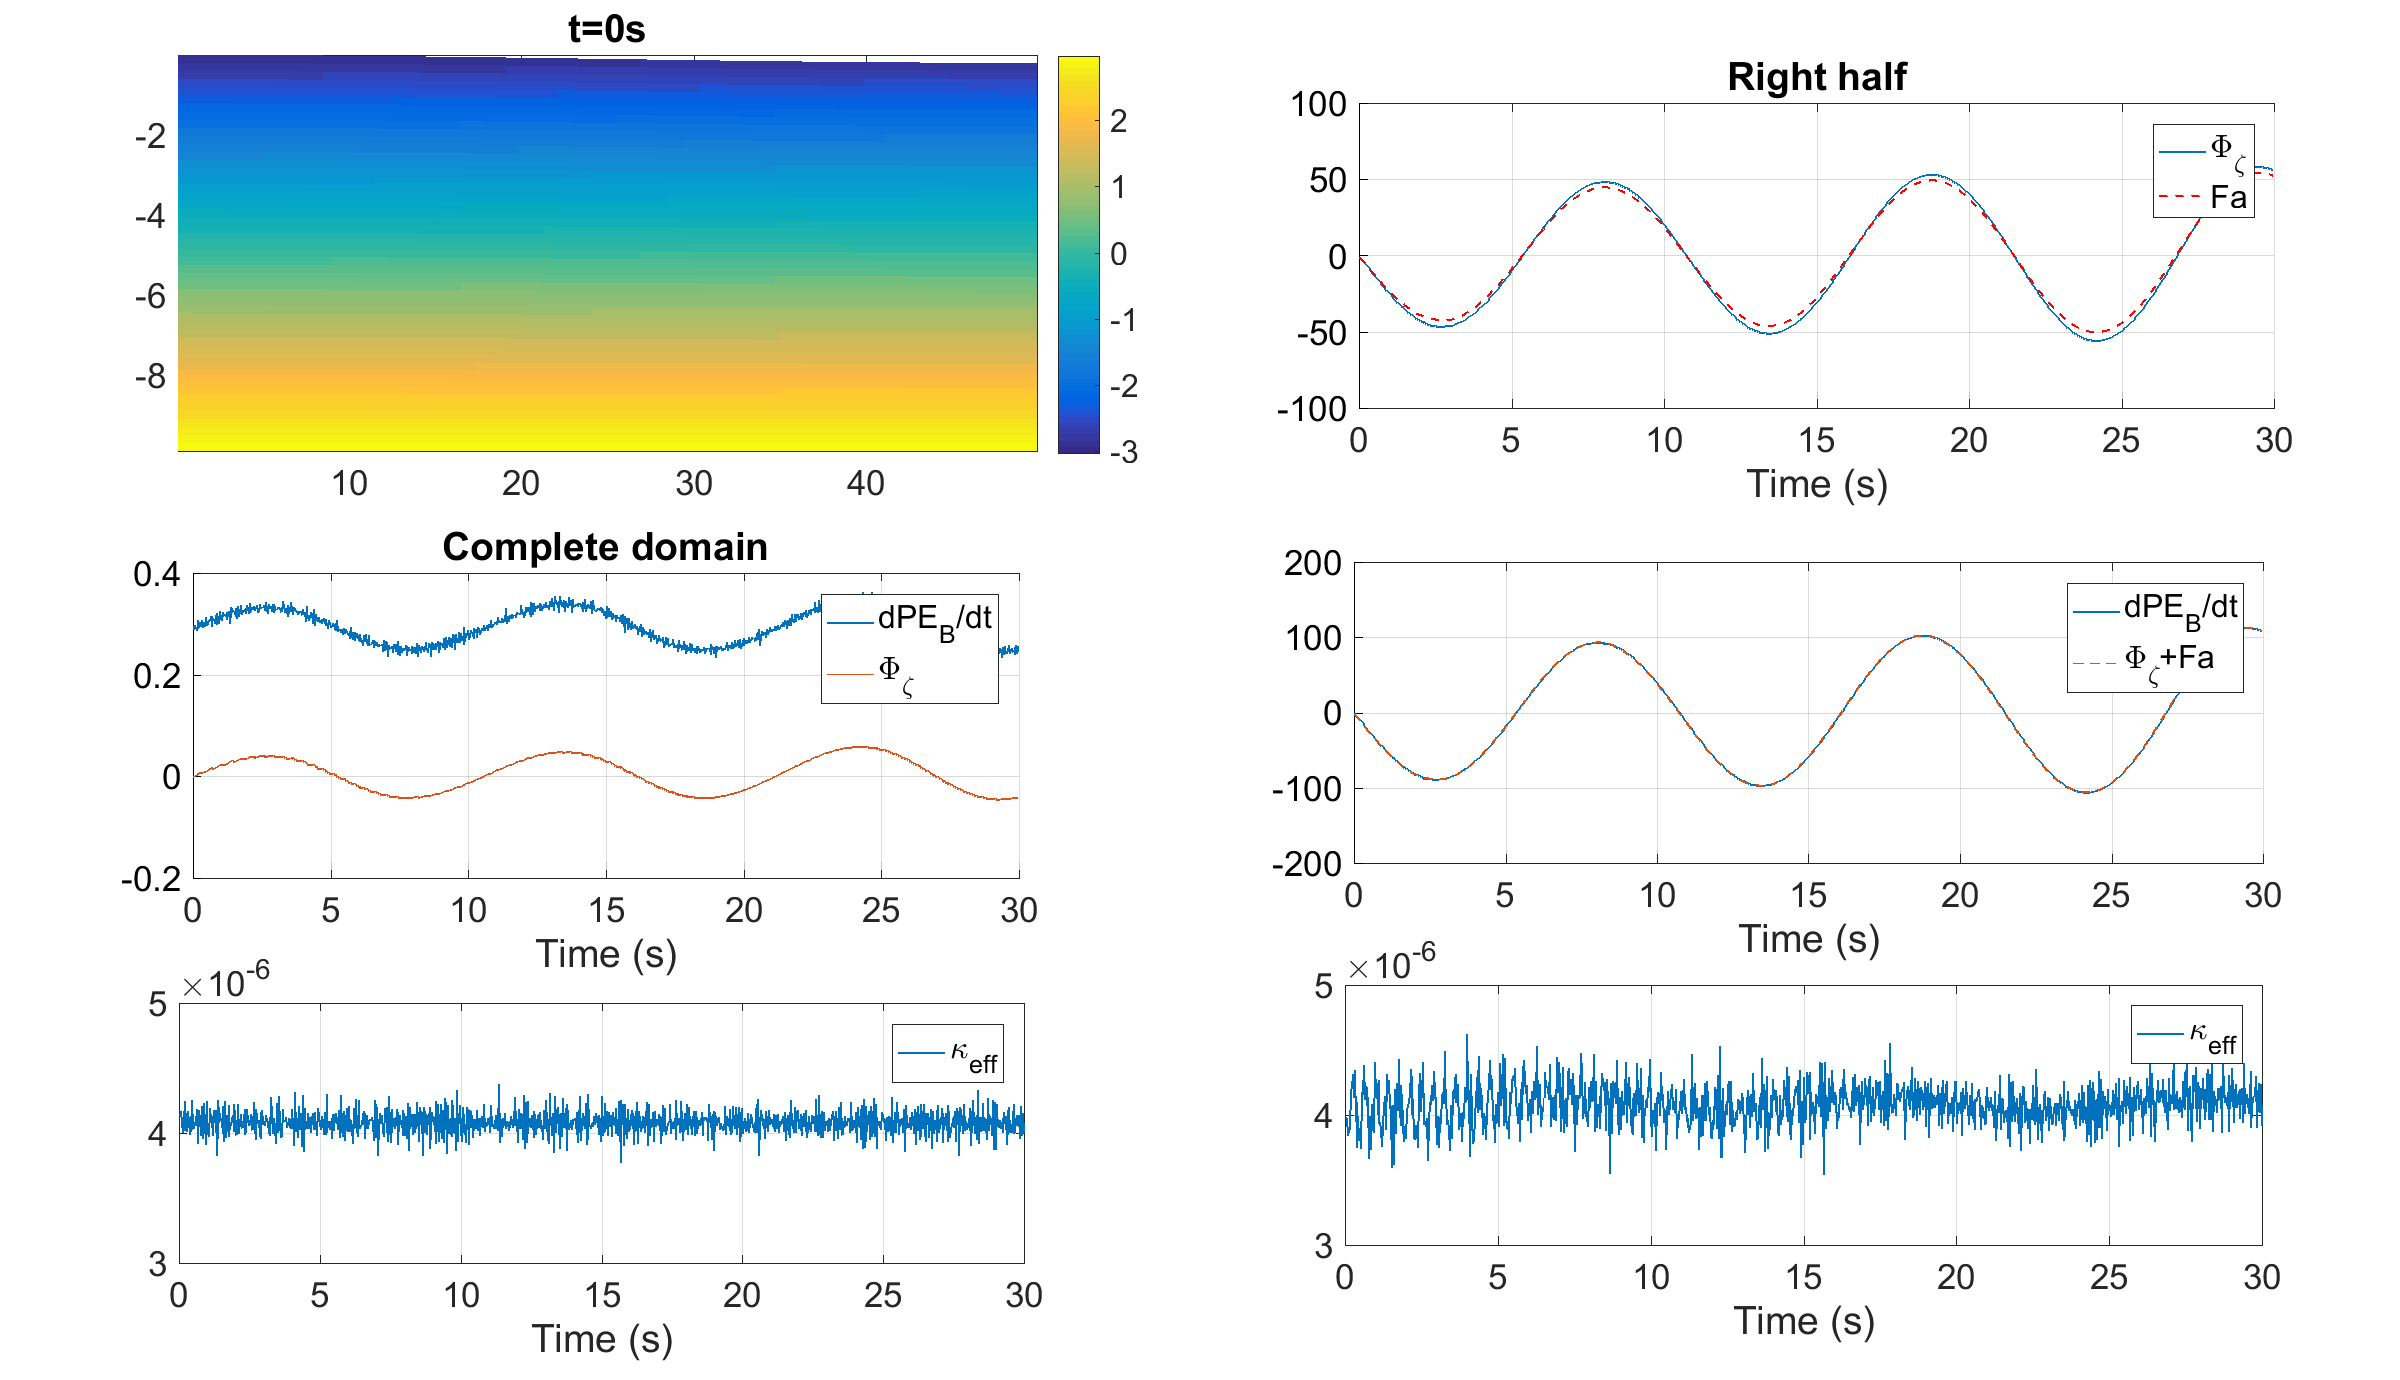
\includegraphics[width=1\textwidth]{./CHAP_BPE/Fig_TANK_linS.png}
\caption{Cas strat lineaire}
\label{figClin}
\end{figure}
%Movement comes from evolution of initially non-flat free surface. Initial linear stratification $\rho(z)$ (ie, constant N) see figure (\noparref{figClin}.A). $\rho_0=1043 kg/m^3$
%\item L$=$50m, H$=$10m, dx$=$0.2m$\approx$dz, amplitude oscillation initiale de la surface libre de 2mm. Explicit diffusion coefficient put at $10^{-4}$m$^2$/s. 
Figure \ref{figClin} shows the initial density field together with the evolution with time of the various terms in the balance equation \ref{bilanBPEal}. Computations are successively carried out for the whole domain (left column of figure \ref{figClin}) or for the right half domain (right column of figure \ref{figClin}).\\
As could be expected, the oscillations of the free-surface clearly governs not only the variations of the first term $(\Phi_{\zeta})$ of this balance equation but also the variations of the overall BPE variations $(dPE_B/dt)$. Indeed, the long-wave phase speed of surface gravity waves $(c\ =\ \sqrt(g L_z)\approx\ 9.9\ m/s)$ induces a natural time-scale of oscillations of the tank of $T_{\zeta}\ =\ L/c\ =\ 5\ s$ when freely propagating from a wall to the other. The period of the oscillations of $dPE_b/dt$ are close to twice $T_{\zeta}$.\\
If the balance equation is evaluated over the whole domain (left column of figure \ref{figClin}), the free-surface term of the evolution equation explains the oscillations of $(dPE_B/dt)$ (figure \noparref{figClin}.c) and the prescribed explicit diffusivity is recovered with good accuracy (figure \noparref{figClin}.e).\\
If the balance equation is now evaluated over the right half domain only (right column of figure \ref{figClin}), $\Phi_{\zeta}$ is approximately equal to $F_a$ the sum of the advective flux trough the (vertical) lateral boundary of this domain (figure \noparref{figClin}.d). Note that the terms of the evolution equation are several orders of magnitude larger than when the balance equation is evaluated over the whole domain. The effective diffusivity is still recovered with good accuracy (figure \noparref{figClin}.f).\\
These results confirms the pertinence of the proposed BPE balance equation (\ref{bilanBPEal}) and reinforces the choices made to evaluate numerically the BPE algorithm. Even in a case where the induced mixing is several order of magnitudes smaller than the other terms of the balance equation, the explicit diffusivity can therefore be recovered both globally and locally based on \ref{eq_kappaEff}.
%If make computation on a half domain $\Phi_{\zeta}$ is of the same amplitude as $F_a$ the advective fluxes. All terms are bigger.
%\item find $\kappa_{eff}$ of the explicit value that was given. Without taking into account $\Phi_{\zeta}$ would have leftover oscillations.

\subsubsection{Pycnocline and free surface ({$BPE_{tank2}$})}
The mixing induced by the natural oscillations of tank are now explored for a two-layer stratification (i.e. for a sharp ocean pycnocline).
\begin{table}[h]
        %\begin{minipage}{.6\textwidth}
        \centering
        \begin{tabular}{|c|c|c|}
                \hline
                Configuration $BPE_{tank2}$ & \textit{Parameters}\\
                \hline 
                Numerical Model & CROCO (compressible, non-hydrostatic kernel)\\
                $L_x$ & 50 m\\
                $L_z$ & 10 m\\
                $\Delta x$ & 0.2 m\\
                $\Delta z$ & $\approx\ 0.2\ m$\\
                $\Delta t$ & Close to CFL requirements in test-configurations.\\
                Diffusivity & $\kappa_{exp} = 10^{-4} \ m^2/s$\\
                \hline
        \end{tabular}
        \captionof{table}{$BPE_{ts2}$ configuration: numerical parameters.}
        \label{tab_BPE_TANK2}
        %\end{minipage}
\end{table}
\begin{figure}[h!]
\centering
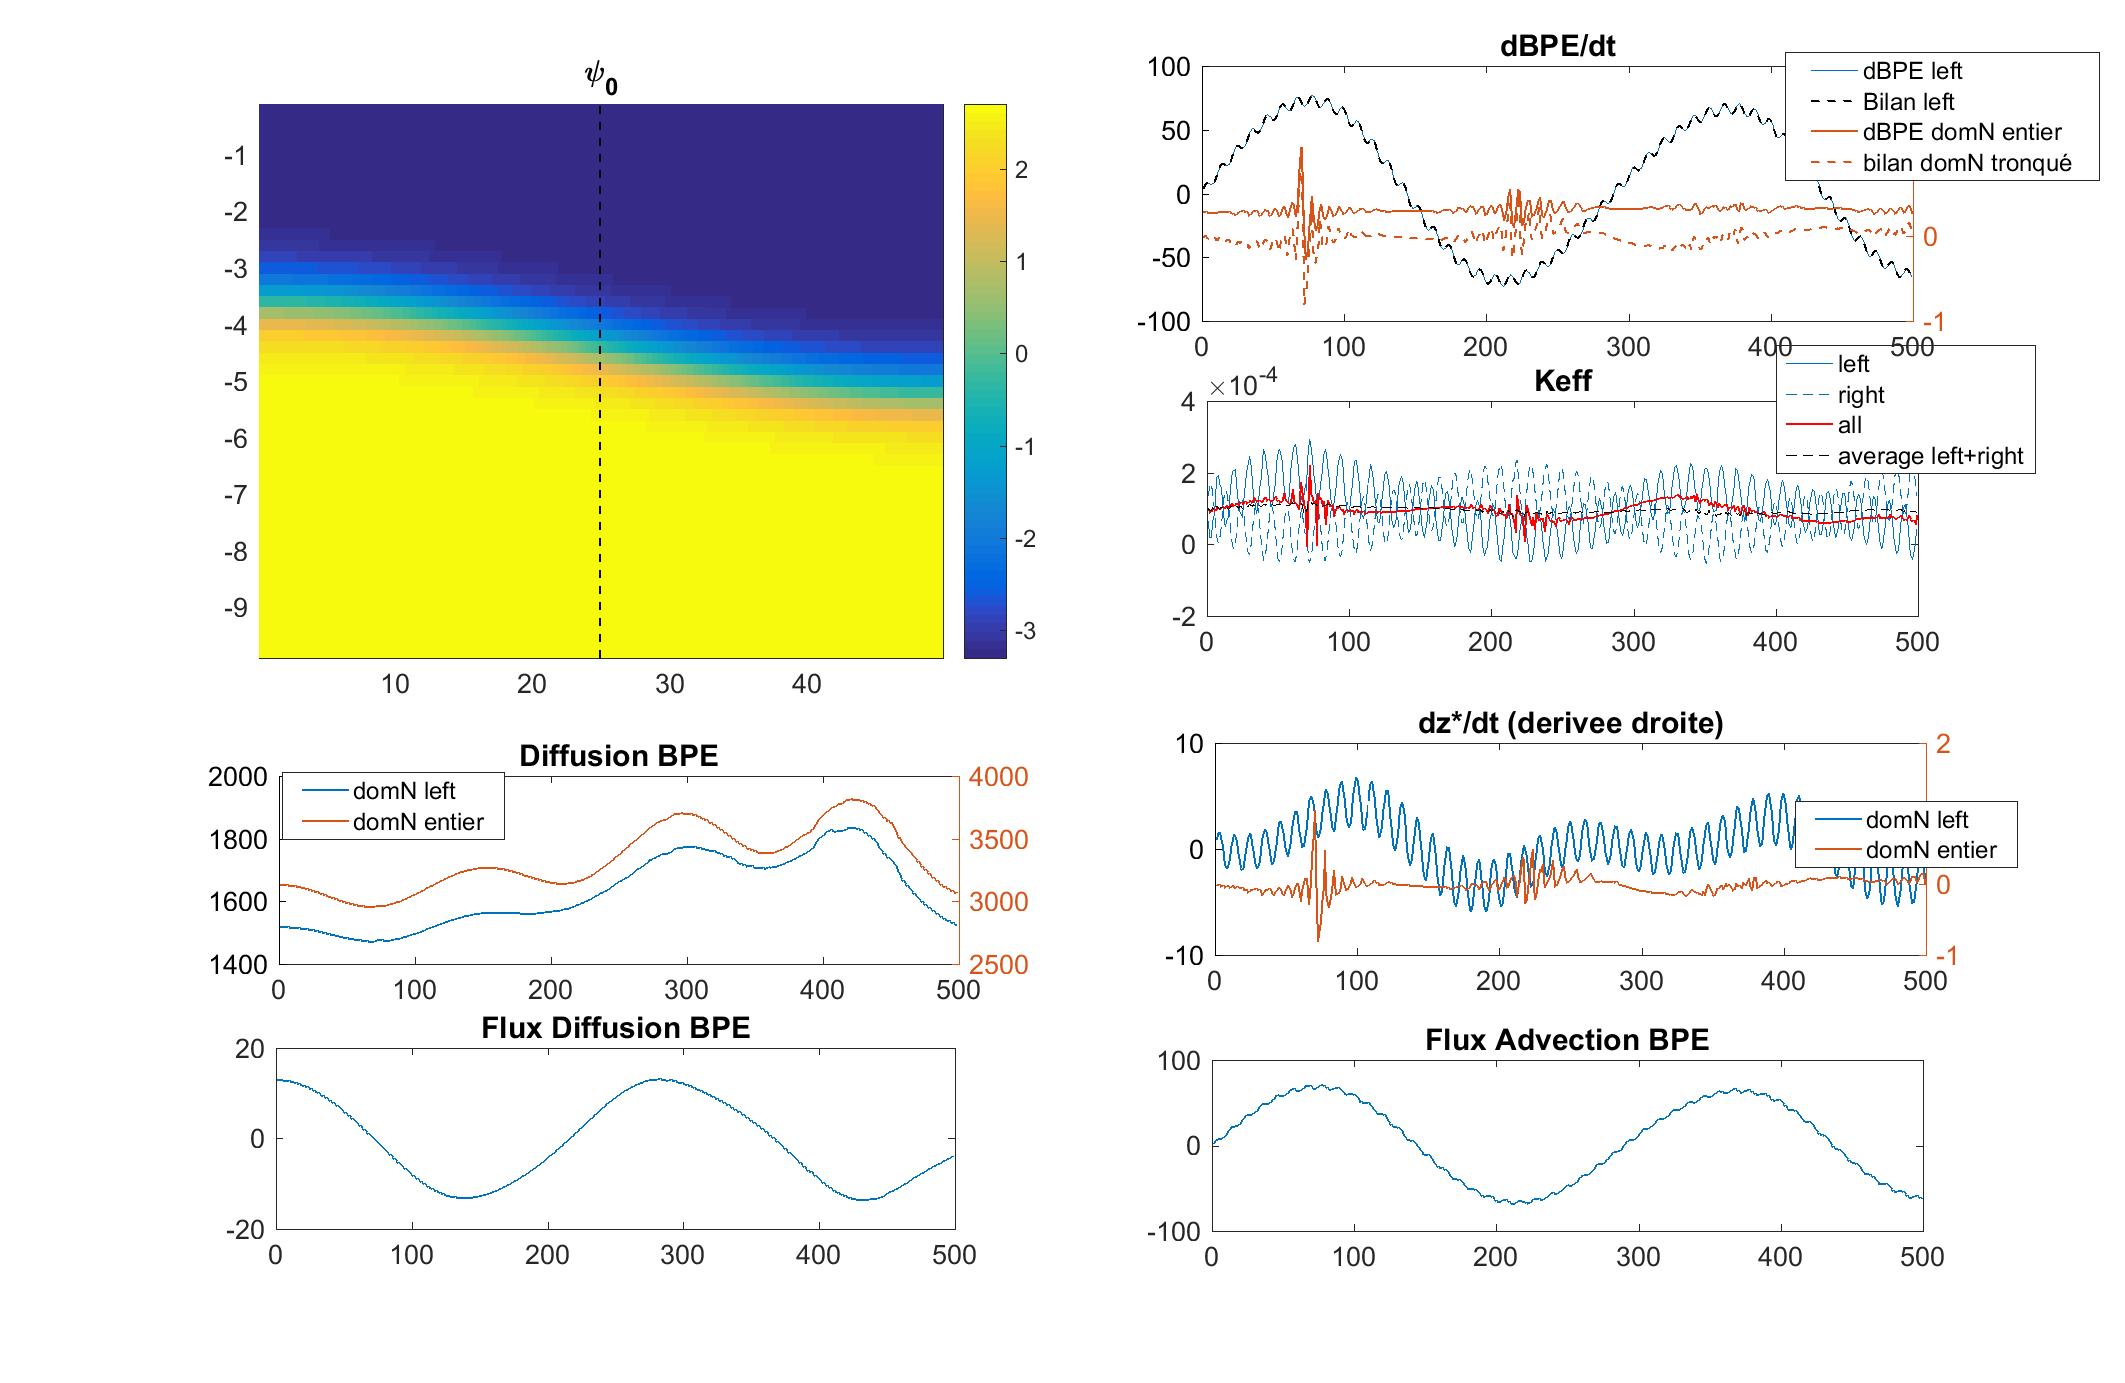
\includegraphics[width=1\textwidth]{./CHAP_BPE/AGBPE_numlab7.png}
\caption{TANK Pycnocline case.bottom row : advection and diffusion flux in regard to the left domain(as discussed in numlab part, do not cancel with fluxes computed for the right half)\color{red}half domain : mettre que un des côtés (?) et faire des moyennes glissante.... Mettre que la figure champ initial et dBPE et Keff\color{black}}
\label{figCpsin}
\end{figure}
Two types of "interfacial" gravity waves can now propagate in this stratified tank: a surface gravity wave with a phase speed of $\sqrt(g L_z) \ \approx \ 9.9\ m/s$ and an internal gravity wave with an interfacial wave speed of $\sqrt(g' h_1 (L_z-h_1)/L_z\ =\ 0.33\ m/s$ ($h_1$ being the depth of the pycnocline). The corresponding time-scales are $T_{\zeta} \ = \ 5 \ s$ and $T_{\eta} \ = \ 150 \ s$.\\
%\item dx$=$dz$=$0.2m, L$=$50m, H$=$10m. Explicit coefficient put at $10^{-4}$m$^2$/s. \color{red}$\rho_0=$\color{black}
%\item Speed surface waves $\sqrt(gH)=5m/s ?????$ and $T_{\zeta}=5s$
%interfacial wave $\sqrt(g'h_1h_2/H)=0.33m/s$ and $T_{\eta}=150s$
The free-surface is supposed to be initially at rest whereas the sinusoidal-shaped initial stratification is shown in figure \ref{figCpsin}.
If the high-frequency oscillations due to the free-surface contribution are filtered out, an increase (decrease) in BPE can be observed in each half domain when the depth of the interface increases (decreases).
%, and respectively BPE will decrease as the interface gets shallower.
Figure \ref{figCpsin} also shows that time-scales associated with the free-surface oscillations do not show up when BPE calculations are carried out over the whole domain but only if they are restricted to half domains. At the opposite, the internal interfacial oscillations can be observed on both type of computations: several pick can even be observed (first at $t\ =\ 80\ s$).
%Otherwise timescale associated with the interface for half domain and also for all the domain. See for all domain a signal (pics a $t=80s$)
%\item note that oscillations in half domain can sometime give a $\kappa_{eff}$ of negative value ( à expliquer... car le prend homogene et isotrope?)
Figure \ref{figCpsin}.c shows the evolution in time of the effective diffusivity when BPE computations are successively carried out over the whole domain (red curve) or over half domains (blue curves). The latter curves present larger-amplitude oscillations but all curves oscillate around the value of the prescribed explicit velocity.

\subsubsection{Pycnocline, free surface and bottom bathymetry}
The last experiment carried out for the tank configuration includes variations of the bathymetry. The objective is to evaluate the limitations of the BPE algorithm for in non-flat domains. The physical and numerical parameters are the same as those given in table \ref{tab_BPE_TANK2} except for the depth which now varies linearly between 10 to 9.25 m. The interfacial internal wave velocity is about $30\ s$.\\
\begin{figure}[h!]
%\begin{subfigure}{.5\textwidth}
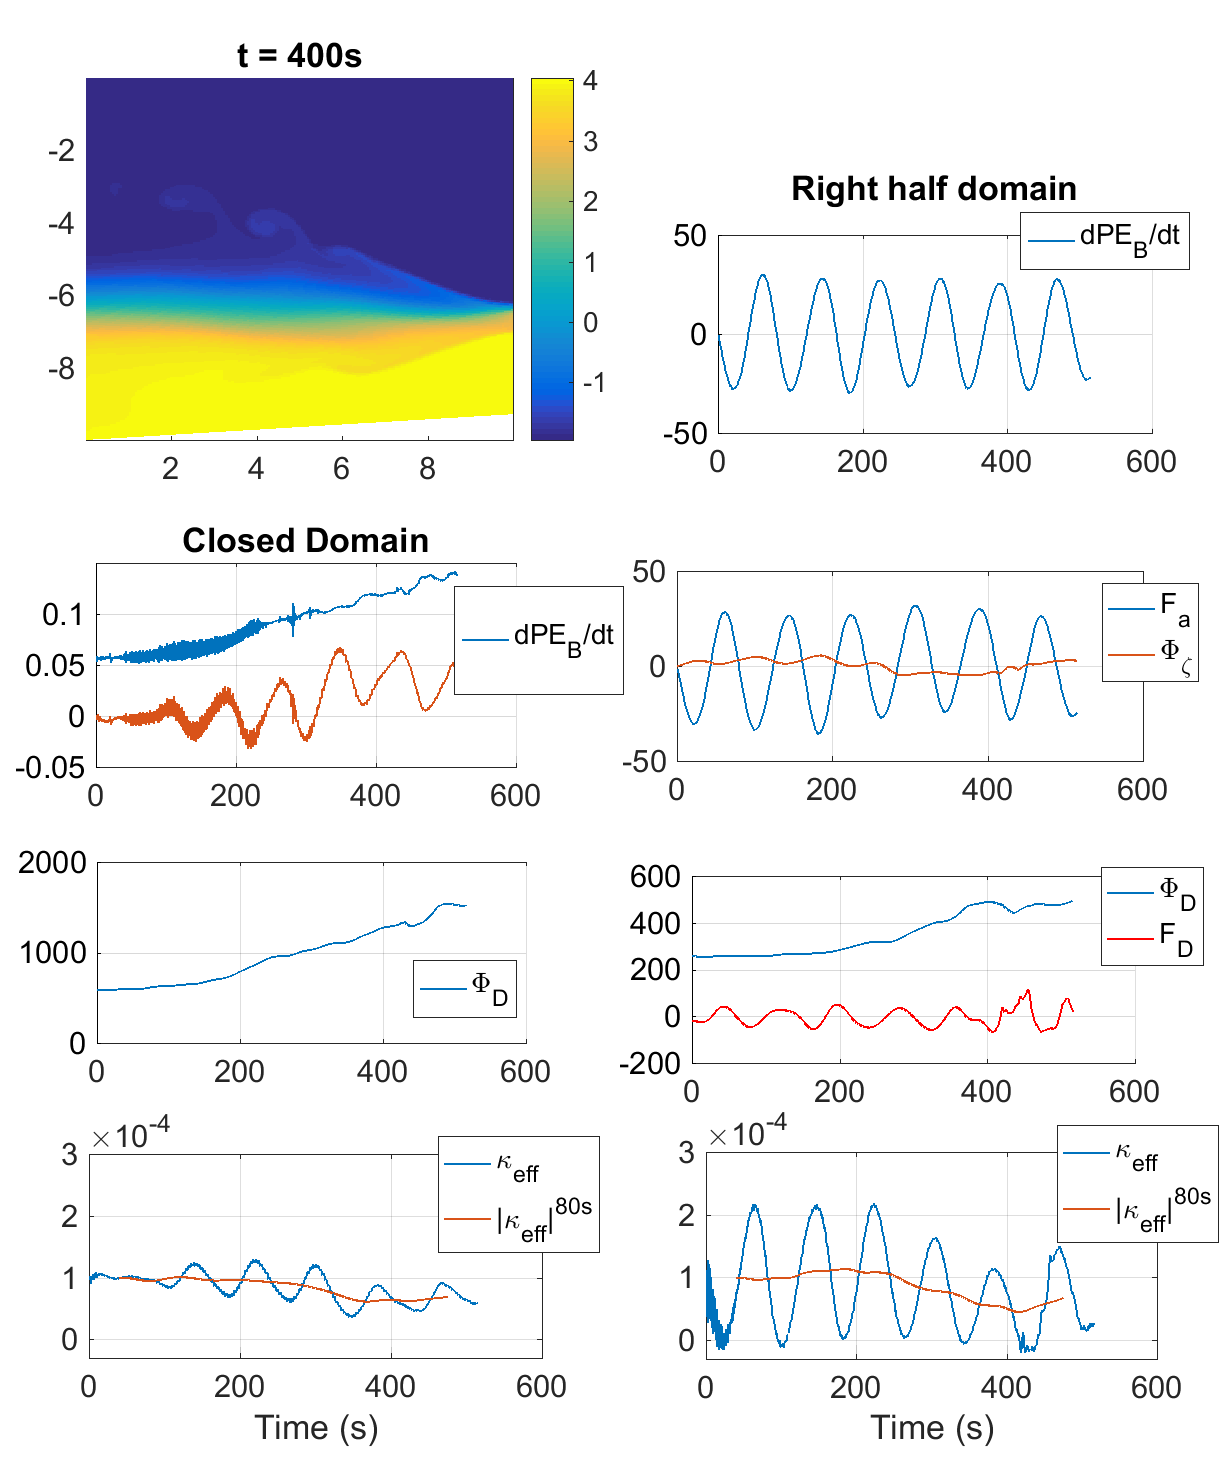
\includegraphics[width=1.\textwidth]{./CHAP_BPE/Fig_TANK_pycbath.png}
%\caption{Closed domain}
%\label{figCkh}
%\end{subfigure}
\caption{Bottom bathy case\color{red}Plus petit\color{black}}
\label{figCbath}
\end{figure}
%\item dx$=$dz$=$0.05m (200 vertical levels), L$=$10m, H$=$10m to 9.25m.$\rho_0=1042 kg/m^3$ Explicit coefficient put at $10^{-4}$m$^2$/s.
%\item Speed of surface waves $\approx 5m/s$,$T_{\zeta}=2s$
The phase speed of internal, interfacial waves is in this case approximately equal to $0.32\ m/s$ and the corresponding time-scale is approximately $T_{\eta}\ =\ 30\ s$\\
In this configuration, the initial slope of the pycnocline leads to Kelvin-Helmholtz instabilities after approximately 6 mn.\\
The BPE evolution equation evaluated over the whole domain shows an increase the variations of both $dPE_B/dt$ and $\phi_D$. The term associated to the free-surface oscillations $(\Phi_{\zeta})$ is shown to oscillate at a period of $80\ s$ which does not correspond to the expected timescale of free-surface oscillations. The same type of oscillations can be observed on the variations of $\kappa_{eff}$. 
The BPE balance equation is evaluated over the right half domain in figure \ref{figCbath} (but a symmetric behaviour can be found for the left half). The advective flux term $(F_a)$ shows larger amplitude oscillations than $\Phi_{\zeta}$ but those oscillations have the same time-scale $(80\ s)$ as the BPE evolution.
%\end{itemize}

%%%%%%%%%%%%%%%%%%%%%%%%%%%%%%%%%%%%%%%%%%%%%
\subsection{Kelvin-Helmholtz Instability ($BPE_{kh}$)}
%\subsubsection{Kelvin-Helmholtz Instability : local estimation and mixing event}
The following configuration focuses on the large turbulent eddies associated to Kelvin-Helmholtz instabilities based on a previous study by \citet{penney_diapycnal_2019}. The corresponding physical and numerical parameters are given in table \ref{tab_BPE_KH}.
\begin{table}[h]
        %\begin{minipage}{.6\textwidth}
        \centering
        \begin{tabular}{|c|c|c|}
                \hline
                Configuration $BPE_{kh}$ & \textit{Parameters}\\
                \hline 
                Numerical Model & CROCO (compressible, non-hydrostatic kernel)\\
                $L_x$ & 256 m\\
                $L_z$ & 256 m\\
                $\Delta x$ & 2 m\\
                $\Delta z$ & $\approx\ 2\ m$\\
                Boundary conditions & Cyclic\\
                $\Delta t$ & Close to CFL requirements in test-configurations.\\
                Diffusivity & $\kappa_{exp} = 10^{-4} \ m^2/s$\\
                \hline
        \end{tabular}
        \captionof{table}{$BPE_{kh}$ configuration: numerical parameters.}
        \label{tab_BPE_KH}
        %\end{minipage}
\end{table}
\begin{figure}[h!]
\centering
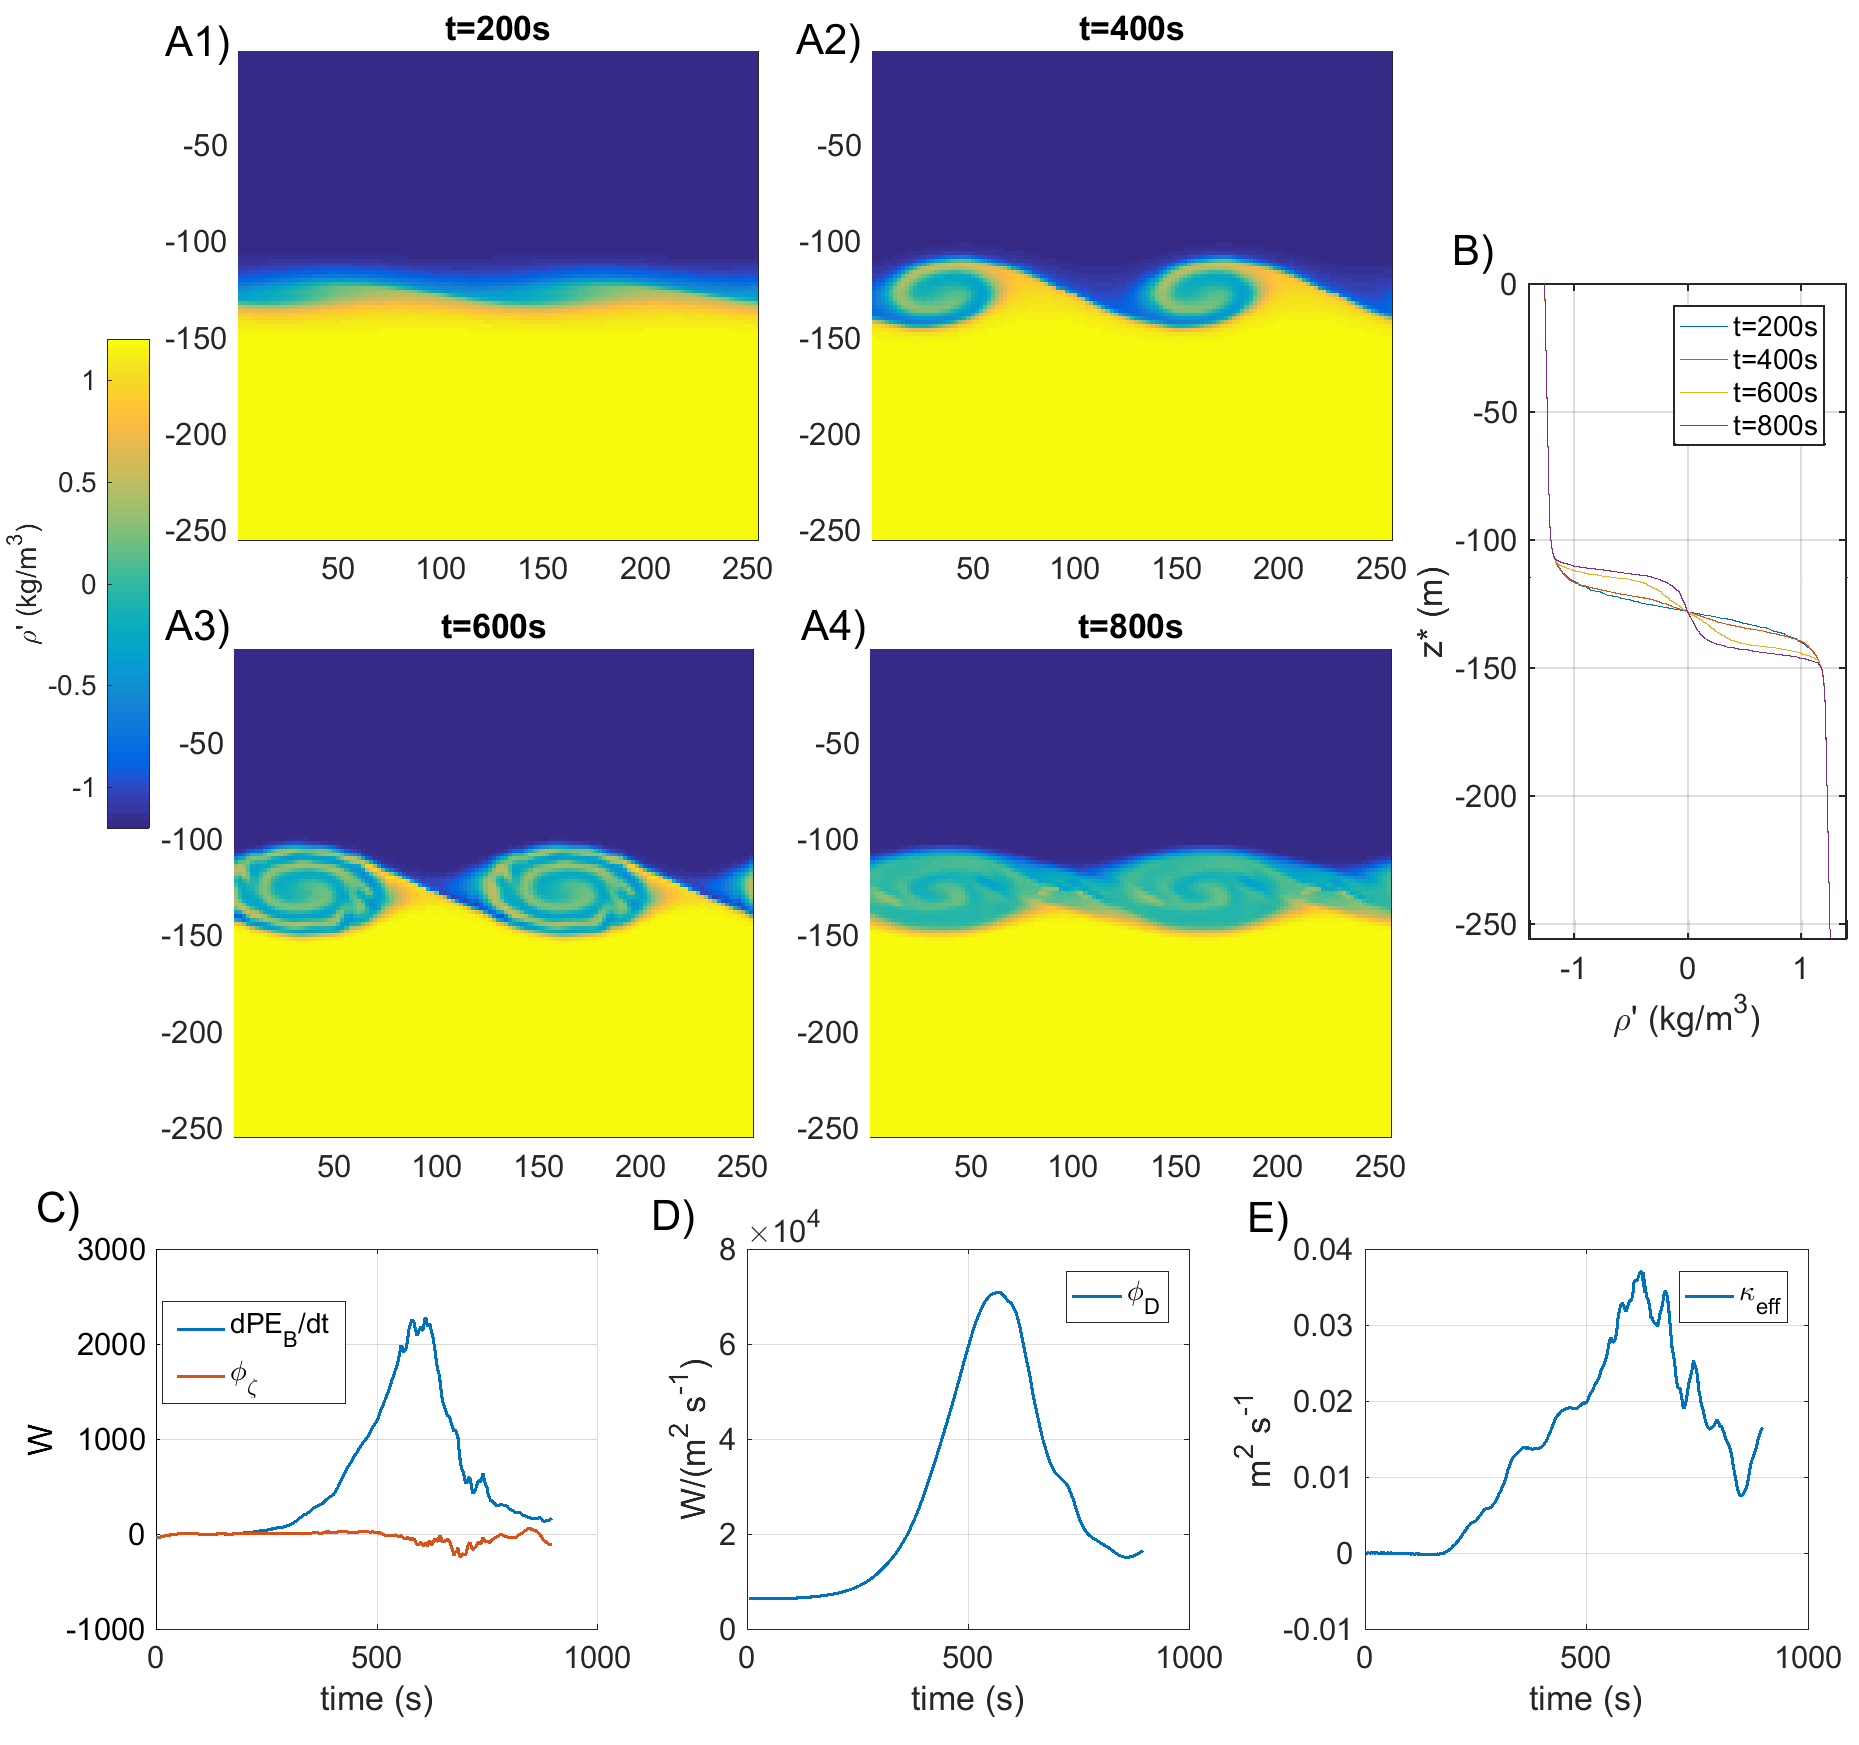
\includegraphics[width=1\textwidth]{./CHAP_BPE/Fig_KH2.png}
\caption{KH testcase}
\label{figCkh}
\end{figure}
% dx$=$dz$=$2m,$\rho_0 = 1034kg/m^3$ ,amplitude cisaillement courant initial 2m/s, cyclic in x, free surface, based on experiments of \citet{penney_2020}.
The initial field is a two-layer stratification  $\Delta \rho\  =\ 2.5\ kg/m^3$ and a two-layer sheared horizontal current with $\Delta U\ =\ 2\ m/s$ in the vertical direction. Two unstable billows develop over the domain during the simulated period.\\
Figure (\noparref{figCkh}.A1-A4) show the evolution of the density field after $t200\ s,\ 400\ s,\ 600\ s$ and $800\ s$ and figure (\noparref{figCkh}.B) gives the evolution of the reference profile at the same times. The figures in the lower row provide the various terms involved in the BPE balance equation \ref{bilanBPEal}.\\
The surface-induced $\phi_{\zeta}$ term remains small compared to the others. The effective diffusivity $\kappa_{eff}$ increases significantly after 200 s as the Kelvin-Helmholtz instability and its associated billows develop. It reaches a maximal value after 600 s which coincides with the maximum amplitude of the diapycnal term $\phi_D$ and the higher shear and density gradients.
Once the Kelvin-Helmholtz instability has mixed the density field, the reference profile exhibits an intermediate homogeneous layer located between $z^*\ =\ 110\ m$ and $z^*\ =\ 140\ m$, which coincides with a decrease of the effective diffusivity $\kappa_{eff}$.

%%%%%%%%%%%%%%%%%%%%%%%%%%%%%%%%%%%%%%%%%%%%%
\subsection{Gibraltar strait configuration ($SimRef$)}
The induced mixing in the vertical section of Gibraltar strait is finally investigated in the simplest configuration of ocean flow in Gibraltar strait (SimRef) originally presented in chapter \ref{chapGBR2D}.\\
\begin{figure}[h!]
\centering
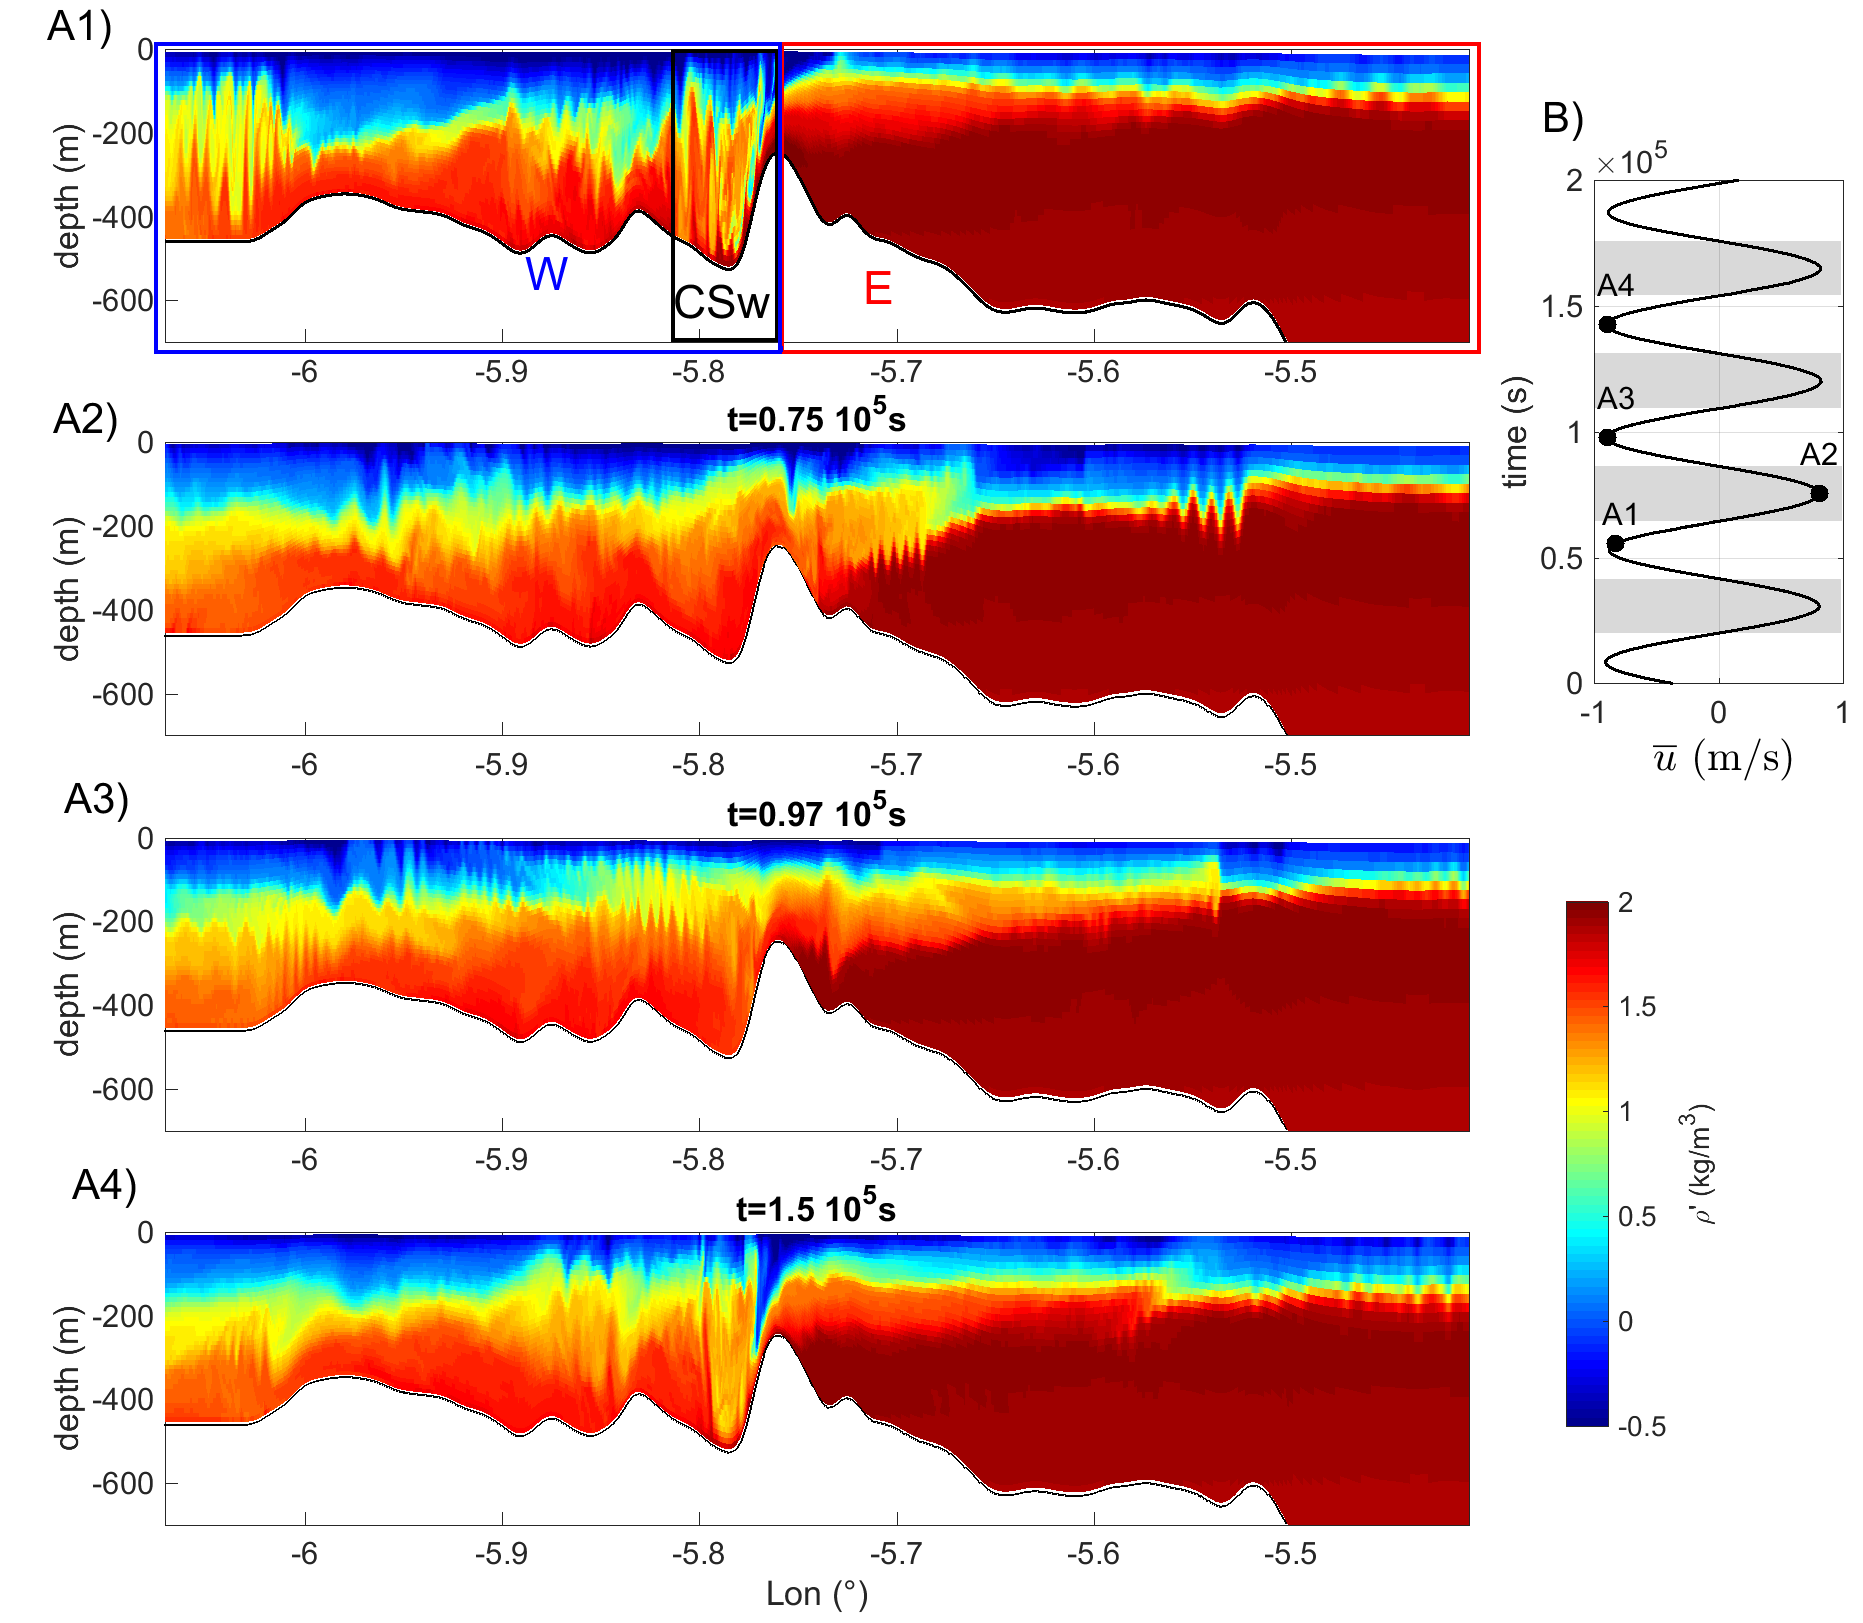
\includegraphics[width=1\textwidth]{./CHAP_BPE/Fig_Kappa_CS_ex.png}
\caption{Definition of domain and snapshots}
\label{figCgbr2d_ex}
\end{figure}
\begin{figure}[h!]
\centering
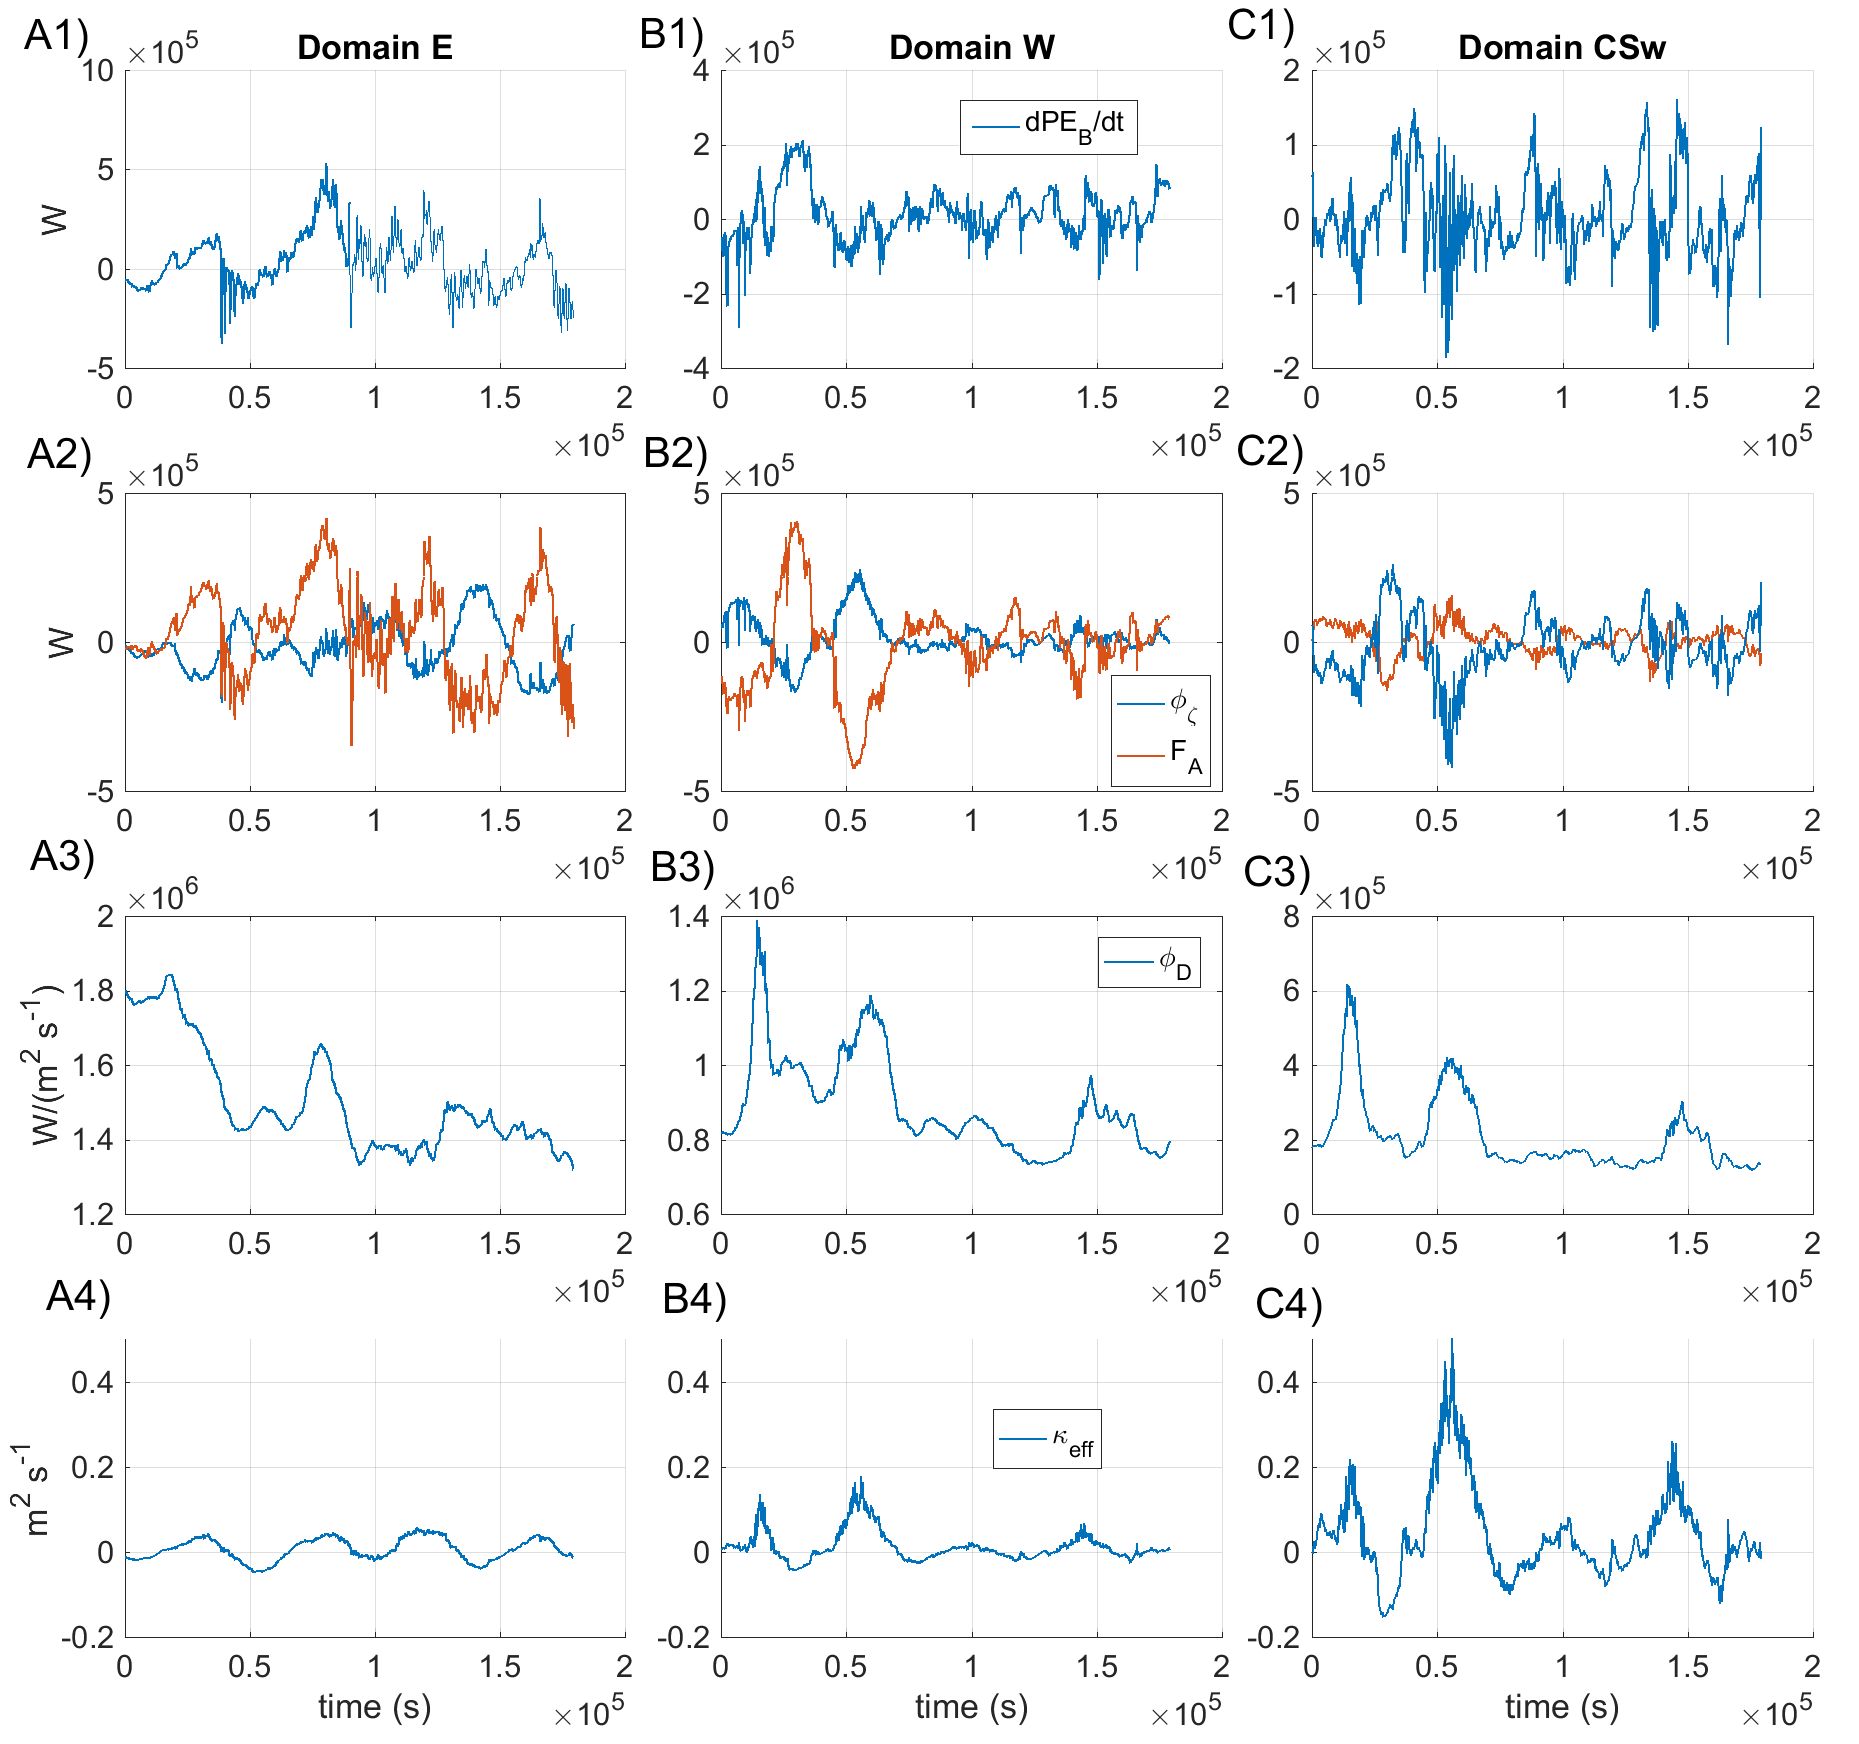
\includegraphics[width=1\textwidth]{./CHAP_BPE/Fig_Kappa_CS.png}
\caption{In each domain}
\label{figCgbr2d}
\end{figure}
The initial time $(t\ =\ 0\ s)$ is now chosen for simulation time $t_{SimRef}\ =\ 6.29\ T$, i.e. at the beginning of the first outflow following the spin-up period whereas the simulation lasts $10.3\ T$ with $T\ =\ 12.4\ h$ the period of semi-diurnal tide.\\
The BPE evolution equation is evaluated over sub-domains of limited extension (see figure \noparref{Fig_Kappa_CS_ex}), where fine-scale processes, large turbulence eddies and thus mixing are supposed to occur. Figure \ref{figCgbr2d} presents the evaluation of the effective diffusivity $\kappa_{eff}$ for each domain, along with the remaining terms of equation \ref{bilanBPEal}.\\ 
The evolution of $dPE_B/dt$ is a noisy signal, the "noise" being largely explained by the sum of the non-diffusive terms $F_a$ and $\phi_{\zeta}$. Those two terms have approximately the same amplitude. Diffusive fluxes through the lateral boundaries are negligible compared to the diapycnal flux $\phi_D$.\\
The evolution in time of the effective diffusivity $\kappa_{eff}$ is in contrast noise-free. In the eastern part of the domain (E), this evolution is sinusoidal of period $T$ in agreement with the evolution of barotropic currents: it is positive positive when the barotropic component of the current is positive.
In the western part of the domain (W) and in it sub-domain (CSw), this semi-diurnal periodicity is readily apparent, not as regular oscillations this time but rather as intermittent episodes (bursts) of higher (positive) effective diffusivity $\kappa_{eff}$ during outflows (when the barotropic component of the current is this time negative).

\section{Discussion and conclusion}
A complete analysis of the Background Potential Energy (BPE) evolution equation has been carried out in several test-configurations of increasing complexity, ending with an application to the real ocean in the region of Gibraltar strait.\\
This analysis is based on original analytical developments (to our knowledge at least) to derive an as-complete-as-possible evolution equation of the Background Potential Energy for free-surface water columns (\S \noparref{section_PE_chap2}). Original developments have also been proposed to evaluate numerically this evolution in non-flat regions of the ocean simulated with terrain-following, s-coordinate numerical models (chapter \noparref{chapBPE}). The efficiency of the proposed implementation of the BPE algorithm remains affordable in terms of computing costs and memory storage for the hierarchy of configurations proposed, but new approaches need to be implemented to compute the reference state \cite{saenz_estimating_2015} for 3D LES of more extended regions.\\
Several assumptions could additionally need to be reconsidered or at least evaluated with care.\\
The isotropy of the effective diffusivity $(\kappa_h=\kappa_v=\kappa)$ should be reconsidered when the implicit numerical diffusion of the advection schemes is at stake: implicit diffusion is indeed added moez specifically along the advection direction and diffusivity is not isotropic anymore.\\
When the reference profile $z^*$ is computed locally, the lateral boundary fluxes exchanged through the vertical boundary separating two neighboring domains do not balance each other. 
The evaluations of the effective diffusivity have been made offline which leads to an additional limitation. Indeed, if an open-boundary configuration is studied, the sampling frequency must be chosen with care and must in particular remain large enough not to induce numerical truncatures or artefacts.\\
In a free-surface domain with opened lateral boundaries, advection and motion of the free surface make $PE_B=\iiint_V \rho g z^* d\tau$ evolve with the reorganisation of the mass field (through $F_a$) and with the change of the water-column volume (through $\phi_{zeta}$). In most studied configurations, those two terms are of the same order of magnitude and are the largest contributions to $dPE_B/dt$. The effective diffusivity $\kappa_{eff}$ is found to complete the balance and thus reflects diapycnal mixing: it quantifies and localizes the averaged turbulent mixing occurring over the domain of integration (a sum of water columns) and over a period which must be long enough for the main underlying dynamical adjustments to be achieved (i.e. at least larger than the time-scale of the diapycnal fluxes).
%\color{red} Here however can see that often find . In open boundary cases especially will have time-evolution appear.\color{black}
%\item The effective diffusivity $\kappa_{eff}$ as an instantaneous, homogeneous, isotropic quantity but mixing can be seen \color{red} plutôt comme gradual process?\color{black}


